\documentclass[11pt,oneside]{article}

\usepackage[a4paper,margin=25mm,headheight=15pt]{geometry}
\usepackage[T1]{fontenc}
\usepackage[utf8]{inputenc}
\IfFileExists{libertinus.sty}{\usepackage{libertinus}}{\usepackage{lmodern}}
\usepackage{microtype}
\usepackage{amsmath,amssymb,amsthm,mathtools,mathrsfs}
\usepackage{bm}
\usepackage{booktabs,longtable,array,tabularx}
\usepackage{graphicx}
\usepackage{xcolor}
\usepackage{enumitem}
\usepackage{fancyhdr}
\usepackage{titlesec}
\usepackage{listings}
\usepackage{xurl}
\usepackage{hyperref}
\usepackage[nameinlink,noabbrev]{cleveref}

\allowdisplaybreaks[2]
\numberwithin{equation}{section}
\setcounter{tocdepth}{2}
\setcounter{secnumdepth}{3}
\setlength{\emergencystretch}{3em}
\graphicspath{{figures/}}

\definecolor{DeepBlue}{HTML}{17365D}
\definecolor{DeepGreen}{HTML}{1D5B45}
\definecolor{DeepRed}{HTML}{8A2D2D}
\definecolor{SoftBlue}{HTML}{EAF1F8}
\definecolor{SoftGreen}{HTML}{EDF7F2}
\definecolor{SoftGray}{HTML}{F4F5F7}
\definecolor{LinkBlue}{HTML}{145DA0}
\definecolor{RuleGray}{HTML}{C5CBD1}

\hypersetup{
  colorlinks=true,
  linkcolor=DeepBlue,
  citecolor=DeepGreen,
  urlcolor=LinkBlue,
  pdftitle={Derivative Norm Spectra and Dual Moment Geometries of the Fabius--Rvachev System},
  pdfauthor={Research report prepared for Vladimir Reshetnikov},
  pdfsubject={Thue--Morse derivative tilings, inverse Fabius beta transforms, Gamma--Bell operators, Stieltjes--Wigert moments, and Lambert endpoint laws},
  pdfkeywords={Fabius function, Rvachev up-function, Thue-Morse, Lp norms, inverse Fabius, Lambert W, Bell polynomials, Bernoulli polynomials, Stieltjes-Wigert, q-binomial, Richardson extrapolation}
}
\urlstyle{same}

\pagestyle{fancy}
\fancyhf{}
\fancyhead[L]{\small Derivative norm spectra}
\fancyhead[R]{\small\nouppercase{\leftmark}}
\fancyfoot[C]{\thepage}
\renewcommand{\headrulewidth}{0.4pt}

\titleformat{\section}{\Large\bfseries\color{DeepBlue}}{\thesection}{0.75em}{}
\titleformat{\subsection}{\large\bfseries\color{DeepBlue}}{\thesubsection}{0.7em}{}
\titleformat{\subsubsection}{\normalsize\bfseries\color{DeepGreen}}{\thesubsubsection}{0.6em}{}

\setlist[itemize]{leftmargin=2em,itemsep=0.25em,topsep=0.4em}
\setlist[enumerate]{leftmargin=2.4em,itemsep=0.25em,topsep=0.4em}

\theoremstyle{plain}
\newtheorem{theorem}{Theorem}[section]
\newtheorem{proposition}[theorem]{Proposition}
\newtheorem{lemma}[theorem]{Lemma}
\newtheorem{corollary}[theorem]{Corollary}
\newtheorem{conjecture}[theorem]{Conjecture}
\theoremstyle{definition}
\newtheorem{definition}[theorem]{Definition}
\newtheorem{algorithm}[theorem]{Algorithm}
\newtheorem{problem}[theorem]{Problem}
\newtheorem{example}[theorem]{Example}
\theoremstyle{remark}
\newtheorem{remark}[theorem]{Remark}
\newtheorem{warning}[theorem]{Warning}

\newcommand{\R}{\mathbb R}
\newcommand{\C}{\mathbb C}
\newcommand{\N}{\mathbb N}
\newcommand{\Z}{\mathbb Z}
\newcommand{\Up}{\operatorname{up}}
\newcommand{\sinc}{\operatorname{sinc}}
\newcommand{\e}{\mathrm e}
\newcommand{\ii}{\mathrm i}
\newcommand{\dd}{\,\mathrm d}
\newcommand{\E}{\mathbb E}
\newcommand{\Prob}{\mathbb P}
\newcommand{\Var}{\operatorname{Var}}
\newcommand{\supp}{\operatorname{supp}}
\newcommand{\sgn}{\operatorname{sgn}}
\newcommand{\dist}{\operatorname{dist}}
\newcommand{\bigO}{\mathcal O}
\newcommand{\smallo}{o}
\newcommand{\Dop}{\mathscr D}
\newcommand{\Mop}{\mathscr M}
\newcommand{\Bop}{\mathscr B}
\newcommand{\qbinom}[3]{\genfrac{[}{]}{0pt}{}{#1}{#2}_{#3}}
\newcommand{\qpoch}[2]{(#1;#2)_\infty}
\newcommand{\qpochfin}[3]{(#1;#2)_{#3}}
\newcommand{\abs}[1]{\left|#1\right|}
\newcommand{\norm}[1]{\left\lVert#1\right\rVert}
\newcommand{\set}[1]{\left\{#1\right\}}
\newcommand{\RepoCommit}{\nolinkurl{0341bbf91cb867f4510bc8431cf59878208de771}}
\newcommand{\RepoRoot}{\url{https://github.com/VladimirReshetnikov/ProveIt/tree/0341bbf91cb867f4510bc8431cf59878208de771/Analysis/FabiusFunction/docs}}

\newenvironment{statusbox}[1]{%
  \par\medskip\noindent\begin{minipage}{\textwidth}%
  \color{DeepBlue}\hrule\vspace{5pt}%
  \color{black}\textbf{\color{DeepBlue}#1.}\ }{%
  \par\vspace{5pt}\color{DeepBlue}\hrule
  \end{minipage}\par\medskip}

\newenvironment{resultbox}[1]{%
  \par\medskip\noindent\begin{minipage}{\textwidth}%
  \color{DeepGreen}\hrule\vspace{5pt}%
  \color{black}\textbf{\color{DeepGreen}#1.}\ }{%
  \par\vspace{5pt}\color{DeepGreen}\hrule
  \end{minipage}\par\medskip}

\newenvironment{conjecturebox}[1]{%
  \par\medskip\noindent\begin{minipage}{\textwidth}%
  \color{DeepRed}\hrule\vspace{5pt}%
  \color{black}\textbf{\color{DeepRed}#1.}\ }{%
  \par\vspace{5pt}\color{DeepRed}\hrule
  \end{minipage}\par\medskip}

\lstdefinestyle{code}{
  basicstyle=\ttfamily\footnotesize,
  backgroundcolor=\color{SoftGray},
  frame=single,
  rulecolor=\color{RuleGray},
  columns=fullflexible,
  keepspaces=true,
  showstringspaces=false,
  breaklines=true,
  xleftmargin=0.6em,
  xrightmargin=0.6em,
  aboveskip=0.8em,
  belowskip=0.8em
}

\title{\bfseries\color{DeepBlue}
Derivative Norm Spectra and Dual Moment Geometries\\[0.25em]
\Large of the Fabius--Rvachev System\\[0.7em]
\large Thue--Morse equimeasurability, inverse-Fabius beta transforms,\\
Gamma--Bell operators, and shifted Stieltjes--Wigert energy measures}
\author{Research report prepared for Vladimir Reshetnikov's \texttt{ProveIt} development}
\date{27 August 2026\\[0.25em]
\small Recursive documentation audit pinned to commit \RepoCommit}

\begin{document}
\maketitle

\begin{abstract}
Let $F$ be the bounded Fabius distribution function, $G=F^{-1}$ its inverse on
$[0,1]$, $\Up(x)=1-F(|x|)$ on $[-1,1]$, and
\[
 \Phi(\xi)=\widehat{\Up}(\xi)
 =\prod_{j=0}^{\infty}\sinc\!\left(\frac{\pi\xi}{2^j}\right)
\]
under the Fourier convention
$\widehat f(\xi)=\int_{\R}f(x)\e^{-2\pi\ii x\xi}\dd x$.
The recursive documentation tree of the \texttt{ProveIt} Fabius development was audited at
commit \RepoCommit.  Existing reports already contain the dyadic derivative tiling,
integer-zero arithmetic, sharp Fourier-decay regimes, endpoint Lambert expansions,
$q$-binomial acceleration, inverse-quantile reversion, and several spectral determinant
constructions.  Those results are treated as baseline rather than renamed.

The first new package extracted here begins with an exact equimeasurability theorem.  If
$T_n=n(n+1)/2$, then $2^{-T_n}|\Up^{(n)}|$ has exactly the same value distribution on
$[-1,1]$ as $\Up$.  The signs on the $2^n$ cells are the length-$2^n$ Thue--Morse block.
Consequently every rearrangement-invariant norm, including every $L^p$ quasi-norm
$0<p\leq\infty$, obeys
\[
 \norm{\Up^{(n)}}_p=2^{T_n}\norm{\Up}_p.
\]
The level sets are also exact:
\[
 \bigl|\{x:\abs{\Up^{(n)}(x)}>2^{T_n}t\}\bigr|=2G(1-t),
 \qquad 0<t<1.
\]
Thus the complete inverse Fabius function is encoded in the value statistics of every
nonzero derivative.

Writing
$A_p=\tfrac12\norm{\Up}_p^p$, one obtains the exact beta transform
\[
 A_p=p\int_0^1(1-y)^{p-1}G(y)\dd y.
\]
For $\Dop=y\,\dd/\dd y$, the dilation variable $Z_p=pY_p$ with
$Y_p\sim\mathrm{Beta}(1,p)$ has Mellin symbol
\[
 \E Z_p^s=p^s\frac{\Gamma(p+1)\Gamma(1+s)}{\Gamma(p+1+s)}.
\]
This yields a new Euler--Gamma differential calculus
\[
 A_p\sim
 G-\gamma\Dop G
 +\frac{\gamma^2+\pi^2/6}{2}\Dop^2G
 -\frac{\gamma^3+\gamma\pi^2/2+2\zeta(3)}{6}\Dop^3G+\cdots
 \quad\text{at }y=p^{-1}.
\]
The coefficients are complete Bell polynomials in log-exponential cumulants; finite-$p$
corrections are generated by Bernoulli polynomials through the gamma-ratio expansion.
Combining this operator with the periodic inverse-Fabius endpoint expansion gives
\[
 \norm{\Up}_p^p
 =2G(p^{-1})\left(1-\frac{\gamma}{\rho}
 +\bigO\!\left(\rho^{-2}\right)\right),
 \qquad
 \rho=\sqrt{\frac{2\log p}{\log2}},
\]
and, more sharply, shows that Euler's constant subtracts from the first periodic inverse
correction.  In particular
\[
 1-\norm{\Up}_p\sim\frac{\sqrt{2\log2\,\log p}}{p}.
\]
A phase-locked sequence of $p$-norms recovers the nonconstant Gamma--zeta endpoint
fluctuation itself.

Parseval turns the same norm law into a second, frequency-side geometry.  The pushforward of
$|\Phi(\xi)|^2\dd\xi/\norm{\Up}_2^2$ by $z=(2\pi\xi)^2$ has moments
\[
 m_n=2^{n(n+1)}=q^{-n(n+1)/2},\qquad q=\frac14.
\]
It is therefore an explicit nonclassical representing measure for a shifted
Stieltjes--Wigert moment problem.  A lognormal measure has the same moments but a different
density, proving indeterminacy directly.  We calculate the Hankel determinants, monic
orthogonal polynomials, recurrence coefficients, and Gaussian-$q$-binomial formulae, and
derive the spectral $q$-Pearson law
\[
 w_{\rm sp}(4z)=\frac12\sinc^2(\sqrt z)\,w_{\rm sp}(z).
\]
The report closes with numerical checks, explicit conjectures, a phase-locked confluent
$q$-Richardson program, and a Lean formalization roadmap.  Claims labelled ``new'' are new
relative to the pinned repository corpus after a formula- and terminology-level collision
audit; no universal publication-priority claim is made.
\end{abstract}

\tableofcontents
\newpage

\section{Scope, corpus audit, and novelty boundary}
\label{sec:scope}

\subsection{What was inspected}

The recursive tree under \RepoRoot{} contained $68$ \texttt{*.tex} artifacts at the pinned
commit.  Every path was included in the audit.  The living expositions, active frontier
reports, Fourier-decay chain, imported paper transcriptions, and mathematically distinctive
archival deltas were read.  The archive deliberately preserves first versions and provenance;
its own ledger explains that byte-identical or superseded descendants should not be treated as
independent contemporary claims.  Accordingly, archived variants were checked for distinctive
content but deduplicated when building the novelty map.  The complete path ledger appears in
\Cref{app:corpus-ledger}.

The most important collision checks were against the following current reports:
\begin{itemize}
\item the primary Fabius--Rvachev exposition and mathematical glossary;
\item the consolidated non-formalized frontier volume;
\item the inverse-frontier report, including periodic Lambert--Bell quantile reversion;
\item the complete Fourier-decay synthesis and its comparative audits;
\item the finite-block/q-Richardson/deconvolution report;
\item the half-integer, arithmetic-ray, spectral determinant, Pascal--Rvachev, and
      Gamma-duality frontier reports;
\item all archived q-calculus, dyadic-asymptotic, Thue--Morse, and repeated-integration
      studies; and
\item the seven imported paper sources.
\end{itemize}

Targeted searches were then run for the exact concepts and formula shapes used below:
``equimeasurable derivative'', ``all-$L^p$ derivative norm'', ``Beta$(1,p)$ inverse
Fabius'', ``$\Gamma(1+\Dop)$'', ``Stieltjes--Wigert'', ``Denjoy--Carleman'', and the exact
moment sequence $2^{n(n+1)}$.  No collision was found for the theorem package developed here.
The underlying derivative tiling itself \emph{is} present in the corpus and is explicitly
marked as baseline.

\subsection{Status convention}

\begin{statusbox}{Three proof-status labels}
\emph{Corpus baseline} means a statement already present, perhaps in another normalization,
in the inspected repository or one of its imported papers.  \emph{New deduction} means a
statement and proof not located in that corpus after the collision audit.  \emph{Conjecture}
means a precise, numerically or structurally motivated statement for which this report does
not claim a proof.  None of these labels asserts global publication priority.
\end{statusbox}

The following are corpus baseline and are not claimed as new:
\begin{enumerate}[label=(\roman*)]
\item the identities relating $F$, $\Up$, and the signed global extension;
\item the differential-refinement law for $\Up$ and its finite Thue--Morse derivative tiling;
\item the infinite sinc product and its integer zero multiplicities;
\item the exact dyadic values of $F$, their $q$-Pochhammer and Gaussian-binomial forms;
\item the corrected endpoint expansion with a nonconstant periodic Gamma--zeta term;
\item the inverse endpoint expansion in the lower-Lambert coordinate, including Bell
      reversion and quantile elasticity;
\item the distinct pointwise, metric, $L^1$, $L^2$, and extremal Fourier-decay exponents;
\item the existing finite-block, q-Richardson, convolution-tail, spectral determinant,
      and Pascal--Rvachev constructions.
\end{enumerate}

\begin{resultbox}{New deductions proved in this report}
The main new results are: exact derivative equimeasurability; scaling in every
rearrangement-invariant norm; exact inverse-Fabius level-set laws; a Hausdorff reconstruction
of $F$ from integer derivative norms; the inverse-Fabius beta transform; an exact Mellin
symbol and asymptotic Euler--Gamma/Bell/Bernoulli differential calculus; a large-$p$
Lambert law with an Euler-constant shift and phase tomography; a shifted
Stieltjes--Wigert spectral-energy measure; explicit Hankel determinants and q-binomial monic
orthogonal polynomials; a nonclassical sinc-square q-Pearson equation; and the exact
Denjoy--Carleman weight and associated periodic Legendre envelope generated by the derivative
norms.
\end{resultbox}

\begin{statusbox}{Post-audit Lean status: a completed derivative-distribution core}
The current source file
\path{Analysis/FabiusFunction/Lean/FabiusFunction/RvachevDerivativeDistribution.lean}
now formalizes the exact dyadic cell coordinate and tiling, every signed cell-midpoint value,
the all-order signed finite-mixture identity for continuous tests with values in an arbitrary
real Banach space, the normalized absolute continuous-test identity, the equality of the two
absolute Borel pushforward measures on Lebesgue measure restricted to \([-1,1]\), and every
nonnegative real absolute moment.  This is a post-audit proof-status update; it does not alter
the pinned novelty comparison above.

The report as a whole is not thereby formalized.  In particular, the simplified signed
Rademacher law as a Borel pushforward, the \path{eLpNorm} and general
rearrangement-invariant norm ladder, the explicit inverse-Fabius level-set laws, the beta
transform and its asymptotics, and all spectral-moment, Hankel, q-Pearson, and
q-binomial layers below remain without matching declarations.
\end{statusbox}

\section{Normalization and established structural identities}
\label{sec:baseline}

Let $F:\R\to[0,1]$ be the bounded Fabius function, with $F=0$ on $(-\infty,0]$,
$F=1$ on $[1,\infty)$, symmetry
\begin{equation}
 F(1-x)=1-F(x),\qquad 0\leq x\leq1,
 \label{eq:F-symmetry}
\end{equation}
and differential law $F'(x)=2F(2x)$ on $0<x<1/2$, continued by symmetry.  Let
\begin{equation}
 \Up(x)=
 \begin{cases}
  1-F(|x|),&|x|\leq1,\\
  0,&|x|\geq1.
 \end{cases}
 \label{eq:up-from-F}
\end{equation}
Then $\Up$ is even, nonnegative, $C^\infty$, supported on $[-1,1]$, satisfies
$\Up(0)=1$ and $\int\Up=1$, and obeys
\begin{equation}
 \Up'(x)=2\bigl(\Up(2x+1)-\Up(2x-1)\bigr).
 \label{eq:up-differential}
\end{equation}
Its Fourier transform is
\begin{equation}
 \Phi(\xi):=\widehat{\Up}(\xi)
 =\prod_{j=0}^{\infty}\sinc\!\left(\frac{\pi\xi}{2^j}\right),
 \qquad \sinc z=\frac{\sin z}{z}.
 \label{eq:phi-product}
\end{equation}

Write
\begin{equation}
 \varepsilon_k:=(-1)^{s_2(k)},\qquad
 T_n:=\binom{n+1}{2}=\frac{n(n+1)}2,
 \label{eq:epsilon-Tn}
\end{equation}
where $s_2(k)$ is the binary digit sum.  The identities
$\varepsilon_{2k}=\varepsilon_k$ and
$\varepsilon_{2k+1}=-\varepsilon_k$ will be used repeatedly.

\begin{theorem}[Corpus baseline: exact derivative tiling]
\label{thm:derivative-tiling}
For every $n\geq0$ and $x\in\R$,
\begin{equation}
 \boxed{
 \Up^{(n)}(x)=2^{T_n}
 \sum_{k=0}^{2^n-1}\varepsilon_k\,
 \Up\!\left(2^n x+2^n-1-2k\right).}
 \label{eq:derivative-tiling}
\end{equation}
Equivalently, for $0\leq k<2^n$ and $-1\leq y\leq1$,
\begin{equation}
 \boxed{
 \Up^{(n)}\!\left(-1+\frac{2k+1+y}{2^n}\right)
 =2^{T_n}\varepsilon_k\Up(y).}
 \label{eq:cell-form}
\end{equation}
\end{theorem}

\begin{proof}
The case $n=0$ is immediate.  Differentiate \eqref{eq:derivative-tiling}.  Each derivative
of an inner copy contributes $2^n$, and \eqref{eq:up-differential} contributes another
factor $2$.  The positive branch has index $2k$ and the negative branch index $2k+1$;
the Thue--Morse identities above give exactly the signs $\varepsilon_{2k}$ and
$\varepsilon_{2k+1}$.  The scalar grows from $2^{T_n}$ to
$2^{T_n+n+1}=2^{T_{n+1}}$.

For the cell form, the support condition
$|2^nx+2^n-1-2j|\leq1$ partitions $[-1,1]$ into the $2^n$ closed cells
\[
 I_{n,k}=\left[-1+\frac{2k}{2^n},-1+\frac{2k+2}{2^n}\right].
\]
On the interior of $I_{n,k}$ only the $k$th summand survives.  At common boundaries every
potentially overlapping copy is evaluated at $\pm1$ and hence vanishes to infinite order.
Solving for the local coordinate gives \eqref{eq:cell-form}.
\end{proof}

\begin{remark}
The corpus already exploits this tiling for derivative values, zeros, and discrete
Thue--Morse structure.  The new step is to view \eqref{eq:cell-form} as a
measure-preserving value-distribution identity and push that observation through normed
function spaces, inverse quantiles, Mellin operators, and spectral moments.
\end{remark}

\begin{statusbox}{Exact Lean parity for the dyadic cells}
The current definition
\path{rvachevDerivativeCell} is exactly
\[
 c_{n,k}(y):=-1+\frac{2k+1+y}{2^n}.
\]
It is total in \(n\) and \(k\).  For \(k<2^n\) it maps \([-1,1]\) into \([-1,1]\);
the first left endpoint is \(-1\), adjacent endpoints agree, and the left endpoint after
all \(2^n\) cells is \(1\).  These facts are
\path{rvachevDerivativeCell_mem_Icc},
\path{rvachevDerivativeCell_zero_neg_one},
\path{rvachevDerivativeCell_one_eq_succ_neg_one}, and
\path{rvachevDerivativeCell_two_pow_neg_one}; the affine dilation about the midpoint is
\path{rvachevDerivativeCell_eq_div_add}.

The signed and absolute formulas \eqref{eq:cell-form} are
\path{iteratedDeriv_rvachev_cell} and
\path{abs_iteratedDeriv_rvachev_cell}.  They include \(n=0\), every valid cell, and both
cell endpoints.  The midpoint specialization
\[
 \Up^{(n)}\!\left(-1+\frac{2k+1}{2^n}\right)
 =2^{T_n}\varepsilon_k
\]
is the separate theorem \path{iteratedDeriv_rvachev_cell_zero}.  All declarations in this
box are in \path{RvachevDerivativeDistribution.lean}.
\end{statusbox}

\section{Exact equimeasurability and the complete derivative norm spectrum}
\label{sec:equimeasurability}

\subsection{Absolute and signed value distributions}

Let $U$ be uniform on $[-1,1]$ and let $R$ be an independent Rademacher variable,
$\Prob(R=1)=\Prob(R=-1)=1/2$.

\begin{theorem}[Derivative equimeasurability]
\label{thm:equimeasurable}
For every $n\geq0$,
\begin{equation}
 \boxed{
 2^{-T_n}\abs{\Up^{(n)}(U)}\ \overset{\mathrm d}=\ \Up(U).}
 \label{eq:absolute-equimeasurable}
\end{equation}
For every $n\geq1$,
\begin{equation}
 \boxed{
 2^{-T_n}\Up^{(n)}(U)\ \overset{\mathrm d}=\ R\Up(U).}
 \label{eq:signed-equimeasurable}
\end{equation}
Equivalently, for every Borel function $H$ for which the integrals exist,
\begin{align}
 \frac12\int_{-1}^{1}H\!\left(2^{-T_n}\abs{\Up^{(n)}(x)}\right)\dd x
 &=\frac12\int_{-1}^{1}H(\Up(y))\dd y,\label{eq:H-absolute}\\
 \frac12\int_{-1}^{1}H\!\left(2^{-T_n}\Up^{(n)}(x)\right)\dd x
 &=\frac14\int_{-1}^{1}\bigl(H(\Up(y))+H(-\Up(y))\bigr)\dd y
 \quad(n\geq1).
 \label{eq:H-signed}
\end{align}
\end{theorem}

\begin{proof}
Integrate cell by cell and use \eqref{eq:cell-form}.  The affine map from each cell to
$[-1,1]$ has Jacobian $2^{-n}$, hence
\[
 \int_{I_{n,k}}H\!\left(2^{-T_n}\abs{\Up^{(n)}(x)}\right)\dd x
 =2^{-n}\int_{-1}^{1}H(\Up(y))\dd y.
\]
Summing $2^n$ equal terms proves \eqref{eq:H-absolute}.  For $n\geq1$, exactly half of the
length-$2^n$ Thue--Morse block has sign $+1$ and half sign $-1$, proving
\eqref{eq:H-signed}.
\end{proof}

\begin{statusbox}{Exact Lean parity for the distribution identities}
The signed theorem presently exposed by Lean is the following all-order finite mixture,
not yet its Rademacher simplification.  If \(E\) is any real Banach space and
\(H:\R\to E\) is continuous, then for every \(n\ge0\),
\begin{equation}
 \int_{-1}^{1}H\!\left(\Up^{(n)}(x)\right)\dd x
 =
 2^{-n}\sum_{k=0}^{2^n-1}
 \int_{-1}^{1}H\!\left(2^{T_n}\varepsilon_k\Up(y)\right)\dd y.
 \label{eq:formal-signed-finite-mixture}
\end{equation}
This is \path{intervalIntegral_comp_iteratedDeriv_rvachev}.  In particular, it includes the
order-zero boundary without introducing a fictitious independent sign.

The same Banach-valued continuous-test API proves
\begin{align}
 \int_{-1}^{1}H\!\left(\abs{\Up^{(n)}(x)}\right)\dd x
 &=
 \int_{-1}^{1}H\!\left(2^{T_n}\Up(y)\right)\dd y,
 \label{eq:formal-absolute-test}\\
 \int_{-1}^{1}H\!\left(2^{-T_n}\abs{\Up^{(n)}(x)}\right)\dd x
 &=
 \int_{-1}^{1}H(\Up(y))\dd y.
 \label{eq:formal-normalized-absolute-test}
\end{align}
These are \path{intervalIntegral_comp_abs_iteratedDeriv_rvachev} and
\path{intervalIntegral_comp_normalized_abs_iteratedDeriv_rvachev}.

More strongly on the absolute side, let
\(\lambda_I\) be Lebesgue measure restricted to \(I=[-1,1]\), and write
\(f_{\#}\mu\) for pushforward.  Lean proves the literal Borel-measure equality
\begin{equation}
 \left(x\longmapsto2^{-T_n}\abs{\Up^{(n)}(x)}\right)_{\#}\lambda_I
 =\Up_{\#}\lambda_I.                                      \label{eq:formal-absolute-pushforward}
\end{equation}
Its declaration is
\path{map_normalized_abs_iteratedDeriv_rvachev_restrict_Icc}.  What is not yet a named
theorem is the signed Borel pushforward simplified, for \(n\ge1\), to
\(R\Up(U)\).  Thus \eqref{eq:signed-equimeasurable} and the full Borel formulation of
\eqref{eq:H-signed} remain on the frontier even though
\eqref{eq:formal-signed-finite-mixture} is their exact continuous-test finite-cell
precursor.
\end{statusbox}

\begin{corollary}[All absolute moments and signed moments]
\label{cor:all-value-moments}
For every real $p\geq0$, interpreting the powers as real powers and using \(0^0=1\) at
\(p=0\),
\begin{equation}
 \int_{-1}^{1}\abs{\Up^{(n)}(x)}^p\dd x
 =\left(2^{T_n}\right)^p\int_{-1}^{1}\Up(x)^p\dd x.
 \label{eq:absolute-moments}
\end{equation}
For every integer $m\geq0$ and $n\geq1$,
\begin{equation}
 \int_{-1}^{1}\Up^{(n)}(x)^m\dd x
 =\begin{cases}
  0,&m\text{ odd},\\
  2^{mT_n}\displaystyle\int_{-1}^{1}\Up(x)^m\dd x,&m\text{ even}.
 \end{cases}
 \label{eq:signed-moments}
\end{equation}
\end{corollary}

The absolute identity \eqref{eq:absolute-moments}, with the exact hypothesis \(p\ge0\), is
\path{intervalIntegral_abs_iteratedDeriv_rvachev_rpow}.  At \(p=0\) this uses Lean's
\path{Real.rpow} convention \(0^0=1\).  The signed parity simplification
\eqref{eq:signed-moments} is not separately formalized.

\subsection{Every rearrangement-invariant norm scales exactly}

A rearrangement-invariant quasi-norm on a finite measure space depends only on the
distribution of $|f|$.  This includes Lebesgue, Lorentz, Lorentz--Zygmund, Orlicz, and many
interpolation spaces.

\begin{theorem}[Universal norm ladder]
\label{thm:universal-norm-ladder}
Let $X[-1,1]$ be any absolutely homogeneous rearrangement-invariant quasi-normed function
space.  Then
\begin{equation}
 \boxed{
 \norm{\Up^{(n)}}_X=2^{T_n}\norm{\Up}_X,
 \qquad n\geq0.}
 \label{eq:RI-norm-law}
\end{equation}
In particular, for every $0<p\leq\infty$,
\begin{equation}
 \boxed{
 \norm{\Up^{(n)}}_{L^p(\R)}
 =2^{n(n+1)/2}\norm{\Up}_{L^p(\R)}.}
 \label{eq:Lp-norm-law}
\end{equation}
\end{theorem}

\begin{proof}
The functions vanish outside $[-1,1]$.  By \Cref{thm:equimeasurable},
$2^{-T_n}|\Up^{(n)}|$ and $\Up$ have the same decreasing rearrangement.  Rearrangement
invariance and absolute homogeneity give \eqref{eq:RI-norm-law}; the $L^p$ case follows.
\end{proof}

\begin{statusbox}{Function-space norm boundary}
The real-power interval identity \eqref{eq:absolute-moments} is formal, but it is not yet
packaged as a Mathlib \path{eLpNorm} equality.  The \(p=\infty\) statement and the general
rearrangement-invariant quasi-norm theorem \eqref{eq:RI-norm-law} likewise have no matching
Lean declarations.  Consequently the universal norm ladder in this subsection remains a
frontier layer; the Borel pushforward equality
\eqref{eq:formal-absolute-pushforward} is its completed measure-theoretic input.
\end{statusbox}

\begin{corollary}[Exact sup norms, total variations, and derivative ratios]
\label{cor:sup-TV}
Since $\norm{\Up}_1=\norm{\Up}_\infty=1$,
\begin{align}
 \norm{\Up^{(n)}}_1&=2^{T_n},\label{eq:L1-exact}\\
 \norm{\Up^{(n)}}_\infty&=2^{T_n},\label{eq:Linf-exact}\\
 \operatorname{TV}(\Up^{(n)})
 =\norm{\Up^{(n+1)}}_1&=2^{T_{n+1}}.
 \label{eq:TV-exact}
\end{align}
For every $0<p\leq\infty$,
\begin{equation}
 \frac{\norm{\Up^{(n+1)}}_p}{\norm{\Up^{(n)}}_p}=2^{n+1}.
 \label{eq:successive-norm-ratio}
\end{equation}
\end{corollary}

\subsection{Thue--Morse extremizers and exact level sets}

\begin{corollary}[Midpoint extrema]
\label{cor:midpoint-extrema}
For $0\leq k<2^n$, put
\begin{equation}
 x_{n,k}:=-1+\frac{2k+1}{2^n}.
 \label{eq:cell-midpoints}
\end{equation}
Then
\begin{equation}
 \boxed{
 \Up^{(n)}(x_{n,k})=2^{T_n}\varepsilon_k.}
 \label{eq:midpoint-values}
\end{equation}
These are precisely the points at which $|\Up^{(n)}|$ attains its global maximum.
Thus the signs of the complete extremal set of the $n$th derivative form the first $2^n$
terms of the signed Thue--Morse sequence.
\end{corollary}

\begin{proof}
Set $y=0$ in \eqref{eq:cell-form} and use $\Up(0)=1$.  Strict decrease of $\Up$ on
$[0,1]$ makes $y=0$ the unique maximum inside each cell.
\end{proof}

The signed midpoint equation \eqref{eq:midpoint-values} is formally
\path{iteratedDeriv_rvachev_cell_zero}.  This does not by itself formalize the exact
inverse-Fabius level sets below.

Let $G=F^{-1}:[0,1]\to[0,1]$.  Since $\Up(y)=1-F(|y|)$,
\begin{equation}
 \set{y\in[-1,1]:\Up(y)>t}=(-G(1-t),G(1-t)),\qquad0<t<1.
 \label{eq:up-level-set}
\end{equation}

\begin{theorem}[Exact inverse-Fabius level-set law]
\label{thm:level-set-law}
For every $n\geq0$ and $0<t<1$,
\begin{equation}
 \boxed{
 \left|\set{x\in\R:
 \abs{\Up^{(n)}(x)}>2^{T_n}t}\right|
 =2G(1-t).}
 \label{eq:derivative-level-set}
\end{equation}
Consequently, if $V_n=2^{-T_n}\abs{\Up^{(n)}(U)}$, then
\begin{align}
 \Prob(V_n>t)&=G(1-t),\label{eq:V-tail}\\
 \Prob(V_n\leq t)&=1-G(1-t),\label{eq:V-cdf}\\
 f_{V_n}(t)&=G'(1-t),\qquad0<t<1.
 \label{eq:V-density}
\end{align}
For $n\geq1$, the signed variable $2^{-T_n}\Up^{(n)}(U)$ has density
\begin{equation}
 f_n(v)=\frac12G'(1-|v|),\qquad-1<v<1.
 \label{eq:signed-value-density}
\end{equation}
\end{theorem}

\begin{proof}
Combine equimeasurability with \eqref{eq:up-level-set}.  The density follows by
differentiating the distribution function on the open interval.  The signed density is the
symmetric Rademacher mixture.
\end{proof}

\begin{statusbox}{Closed-form level-set boundary}
Equation \eqref{eq:formal-absolute-pushforward} proves exact absolute equimeasurability as
a Borel measure identity.  The further identifications
\eqref{eq:derivative-level-set}--\eqref{eq:signed-value-density}, which express the sets
and densities explicitly through the totalized inverse \(G\), do not yet have matching Lean
theorems.  In particular, the exact level-set and density package remains unformalized.
\end{statusbox}

\begin{remark}[A quantile coupling]
If $U$ is uniform on $[-1,1]$, then $|U|$ is uniform on $[0,1]$ and
\begin{equation}
 G\!\left(1-\Up(U)\right)=|U|.
 \label{eq:quantile-coupling}
\end{equation}
Thus the inverse Fabius function is not merely asymptotically related to derivative values;
it is their exact probability integral transform.
\end{remark}

\section{The norm spectrum determines the Fabius function}
\label{sec:hausdorff}

Define the normalized norm spectrum
\begin{equation}
 A_p:=\frac12\norm{\Up}_p^p
 =2^{-1-pT_n}\norm{\Up^{(n)}}_p^p,
 \qquad p>0.
 \label{eq:Ap-definition}
\end{equation}
The second expression is independent of $n$ by \eqref{eq:Lp-norm-law}.
Set $A_0:=1$.  If $W=\Up(U)$, then $A_p=\E W^p$ for every $p\geq0$.

\begin{proposition}[Complete monotonicity and log-convexity]
\label{prop:complete-monotonicity}
The function $p\mapsto A_p$ is strictly completely monotone on $(0,\infty)$:
\begin{equation}
 (-1)^rA_p^{(r)}
 =\E\bigl[W^p(-\log W)^r\bigr]>0,
 \qquad r\geq0.
 \label{eq:continuous-complete-monotonicity}
\end{equation}
It is strictly log-convex.  Its integer samples are a completely monotone Hausdorff moment
sequence:
\begin{equation}
 (-1)^r\Delta^r A_m
 =\E\bigl[W^m(1-W)^r\bigr]>0,
 \qquad m,r\geq0,
 \label{eq:discrete-complete-monotonicity}
\end{equation}
where $\Delta A_m=A_{m+1}-A_m$.
\end{proposition}

\begin{proof}
Write $W^p=\exp(-pX)$ with $X=-\log W\geq0$ and differentiate under the integral.
Strict log-convexity follows from H\"older's inequality because $W$ is nonconstant.
The finite-difference formula follows by expanding $(1-W)^r$.
\end{proof}

\begin{theorem}[Hausdorff reconstruction from integer derivative norms]
\label{thm:hausdorff-reconstruction}
The sequence $\{A_m\}_{m\geq0}$ uniquely determines $G$, hence $F$ and $\Up$.
More explicitly, define
\begin{equation}
 b_{N,k}:=\binom Nk
 \sum_{j=0}^{N-k}(-1)^j\binom{N-k}{j}A_{k+j},
 \qquad0\leq k\leq N.
 \label{eq:bernstein-masses}
\end{equation}
Then $b_{N,k}\geq0$, $\sum_kb_{N,k}=1$, and at every $0<t<1$,
\begin{equation}
 \boxed{
 G(1-t)=1-\lim_{N\to\infty}
 \sum_{k=0}^{\lfloor Nt\rfloor}b_{N,k}.}
 \label{eq:G-from-norms}
\end{equation}
The same reconstruction applies to the normalized norms of any fixed derivative
$\Up^{(n)}$ through \eqref{eq:Ap-definition}.
\end{theorem}

\begin{proof}
By \eqref{eq:discrete-complete-monotonicity},
\[
 b_{N,k}=\binom Nk\E\bigl[W^k(1-W)^{N-k}\bigr].
\]
Conditioned on $W=w$, these are the probabilities of a binomial random variable
$K_N\sim\operatorname{Bin}(N,w)$.  Therefore
\[
 \sum_{k=0}^{\lfloor Nt\rfloor}b_{N,k}
 =\E\Prob(K_N/N\leq t\mid W).
\]
The conditional law of large numbers makes the inner probability converge to
$\mathbf1_{\{W\leq t\}}$ away from $w=t$.  The distribution of $W$ is continuous, so the
expectation converges to $\Prob(W\leq t)=1-G(1-t)$ by
\eqref{eq:V-cdf}.  Uniqueness is also the classical determinacy of the Hausdorff moment
problem on $[0,1]$.
\end{proof}

\begin{remark}
This theorem gives a perhaps unexpected completeness statement: the scalar sequence
$\norm{\Up^{(n)}}_m$, $m=1,2,\ldots$, for any one derivative order $n$, contains the entire
Fabius function.  The Thue--Morse oscillation disappears under absolute moments, yet no
information about the underlying profile is lost.
\end{remark}

\section{An exact inverse-Fabius beta transform}
\label{sec:beta-transform}

\begin{theorem}[Beta transform of the inverse Fabius function]
\label{thm:beta-transform}
For every real $p>0$,
\begin{equation}
 \boxed{
 A_p=p\int_0^1(1-y)^{p-1}G(y)\dd y.}
 \label{eq:beta-transform}
\end{equation}
Equivalently, if $Y_p\sim\operatorname{Beta}(1,p)$, then
\begin{equation}
 \boxed{A_p=\E G(Y_p).}
 \label{eq:beta-expectation}
\end{equation}
\end{theorem}

\begin{proof}
Using evenness and \eqref{eq:up-from-F},
\[
 A_p=\int_0^1(1-F(x))^p\dd x.
\]
The monotone substitution $y=F(x)$, interpreted as a Lebesgue--Stieltjes substitution at the
flat endpoints, gives
\[
 A_p=\int_0^1(1-y)^p\dd G(y).
\]
Integration by parts has no boundary term because $G(0)=0$ and $(1-y)^p=0$ at $y=1$.
This proves \eqref{eq:beta-transform}; the beta density is
$p(1-y)^{p-1}$.
\end{proof}

\begin{corollary}[Layer-cake form]
For every $p>0$ and every $n\geq0$,
\begin{equation}
 \norm{\Up^{(n)}}_p^p
 =2^{pT_n+1}p\int_0^1(1-y)^{p-1}G(y)\dd y.
 \label{eq:derivative-beta-transform}
\end{equation}
\end{corollary}

The beta kernel concentrates at $y\asymp p^{-1}$.  Because $G$ is slowly varying at zero,
\eqref{eq:beta-transform} already implies $A_p\sim G(1/p)$.  The next section replaces that
first-order Abelian statement by an all-orders differential operator.

\section{The Euler--Gamma differential operator}
\label{sec:gamma-operator}

\subsection{Exact Mellin symbol}

Let
\begin{equation}
 \Dop:=y\frac{\dd}{\dd y}
 \label{eq:Euler-operator}
\end{equation}
be the Euler dilation derivative.  Put $Z_p=pY_p$.

\begin{proposition}[Mellin symbol of the beta dilation]
\label{prop:Mellin-symbol}
For $\Re s>-1$,
\begin{equation}
 \boxed{
 M_p(s):=\E Z_p^s
 =p^s\frac{\Gamma(p+1)\Gamma(1+s)}{\Gamma(p+1+s)}.}
 \label{eq:Mellin-symbol}
\end{equation}
For any bounded extension of $G$ to $(1,\infty)$,
\begin{equation}
 \boxed{
 A_p=\left[M_p(\Dop)G\right](p^{-1}),}
 \label{eq:exact-operator}
\end{equation}
where the operator is rigorously interpreted by the Bochner average
\begin{equation}
 \left[M_p(\Dop)H\right](y)
 :=\E\left[H(Z_py)\right].
 \label{eq:Bochner-dilation}
\end{equation}
The value in \eqref{eq:exact-operator} is independent of how $G$ is extended, because
$0<Z_p/p=Y_p<1$.
\end{proposition}

\begin{proof}
The beta integral gives
\[
 \E Z_p^s=p^s p\int_0^1y^s(1-y)^{p-1}\dd y
 =p^s\frac{\Gamma(p+1)\Gamma(1+s)}{\Gamma(p+1+s)}.
\]
The dilation semigroup satisfies $\exp(t\Dop)H(y)=H(\e^t y)$.  Averaging with
\(t=\log Z_p\) and evaluating at $y=p^{-1}$ gives
$\E G(Z_p/p)=\E G(Y_p)=A_p$.
\end{proof}

As $p\to\infty$, $Z_p$ converges to an exponential random variable $Z$ of mean one, and
$M_p(s)\to\Gamma(1+s)$.  Thus $\Gamma(1+\Dop)$ is not decorative notation: it is the Mellin
symbol of the limiting random dilation.

\subsection{Cumulants, Bell polynomials, and finite-p corrections}

Let
\begin{equation}
 K_p(s):=\log M_p(s).
 \label{eq:Kp}
\end{equation}
The cumulants of $\log Z_p$ are
\begin{align}
 \kappa_{1,p}&=\log p-\psi(p+1)-\gamma,
 \label{eq:kappa1p}\\
 \kappa_{m,p}&=\psi^{(m-1)}(1)-\psi^{(m-1)}(p+1),
 \qquad m\geq2.
 \label{eq:kappamp}
\end{align}
If $B_m$ denotes the complete exponential Bell polynomial, then
\begin{equation}
 \mu_{m,p}:=\E(\log Z_p)^m
 =B_m(\kappa_{1,p},\ldots,\kappa_{m,p}).
 \label{eq:log-moments-Bell}
\end{equation}
As $p\to\infty$,
\begin{align}
 \kappa_1&=-\gamma,\label{eq:kappa-limit-1}\\
 \kappa_m&=(-1)^m(m-1)!\zeta(m),\qquad m\geq2,
 \label{eq:kappa-limit-m}
\end{align}
which are the cumulants of $\log Z$ for $Z\sim\operatorname{Exp}(1)$.

The uniform gamma-ratio expansion on compact $s$-sets is
\begin{equation}
 \boxed{
 K_p(s)\sim\log\Gamma(1+s)
 +\sum_{r=1}^{\infty}
 \frac{(-1)^{r+1}\bigl(B_{r+1}(1)-B_{r+1}(1+s)\bigr)}
 {r(r+1)p^r}.}
 \label{eq:Bernoulli-gamma-ratio}
\end{equation}
Here $B_m(x)$ are Bernoulli polynomials.  The first correction is
$-s(s+1)/(2p)$.

\begin{theorem}[Local Gamma--Bell expansion]
\label{thm:Gamma-Bell-expansion}
Fix $N\geq1$.  As $p\to\infty$,
\begin{equation}
 \boxed{
 A_p=
 \sum_{m=0}^{N-1}\frac{\mu_m}{m!}
 \Dop^mG(p^{-1})
 +\bigO_{N}\!\left(
 G(p^{-1})\frac{(\log\rho)^{c_N}}{\rho^N}
 \right),}
 \label{eq:Gamma-Bell-expansion}
\end{equation}
where
\begin{equation}
 \rho=\sqrt{\frac{2\log p}{\log2}},
 \qquad
 \mu_m=B_m\bigl(-\gamma,\zeta(2),-2\zeta(3),6\zeta(4),\ldots\bigr),
 \label{eq:mu-limit}
\end{equation}
and $c_N$ is a finite integer depending only on $N$.
A finite-$p$ expansion with corrections to every power of $p^{-1}$ is obtained by replacing
$\mu_m$ with \eqref{eq:log-moments-Bell} or, equivalently, substituting
\eqref{eq:Bernoulli-gamma-ratio} into $\exp K_p(\Dop)$.
\end{theorem}

\begin{proof}
Write $y=p^{-1}$ and $t=\log Z_p$.  On a logarithmic neighborhood of $y$,
\[
 G(\e^t y)=\sum_{m=0}^{N-1}\frac{t^m}{m!}\Dop^mG(y)+R_N(t,y).
\]
The all-orders inverse endpoint expansion in the corpus implies, for each fixed $m$,
$\Dop^mG(y)/G(y)$ is bounded by a power of $\log\rho$ times $\rho^{-m}$.
Fix a constant $C>L+1$ and split the expectation into $|t|\leq C\rho$ and its complement.
On the central range, every point $\e^u y$ between $y$ and $\e^t y$ has endpoint coordinate
$\rho+\bigO_C(1)$.  Integrating the elasticity shows
$G(\e^u y)/G(y)=\bigO_C(1)$ there, so Taylor's integral remainder is
\[
 |R_N(t,y)|\leq C_NG(y)\frac{(\log\rho)^{c_N}}{\rho^N}|t|^N.
\]
The moments $\E|\log Z_p|^N$ are bounded uniformly for $p\geq2$: near zero the density of
$Z_p$ is at most one, while for $z\geq1$ it is bounded by $\e^{-z/2}$.
For the omitted negative tail,
$\Prob(Z_p<\e^{-C\rho})\leq\e^{-C\rho}$; for the positive tail,
$\Prob(Z_p>\e^{C\rho})\leq\exp(-\e^{C\rho})$ once $p$ is large.  Since
$G(p^{-1})\asymp\rho\e^{-L\rho}$, both tail contributions are
$\smallo(G(p^{-1})\rho^{-N})$.  Taking expectations gives coefficients $\mu_{m,p}$;
replacing them by $\mu_m$ changes the result by $\bigO(p^{-1}G(p^{-1}))$, which is beyond
every power of $\rho^{-1}$ relative to $G(p^{-1})$.  The Bell and Bernoulli descriptions
follow from differentiation of \eqref{eq:Kp} and the standard gamma-ratio expansion.
\end{proof}

The first five log-exponential moments are
\begin{align}
 \mu_0&=1,\nonumber\\
 \mu_1&=-\gamma,\nonumber\\
 \mu_2&=\gamma^2+\zeta(2),\nonumber\\
 \mu_3&=-\gamma^3-3\gamma\zeta(2)-2\zeta(3),\nonumber\\
 \mu_4&=\gamma^4+6\gamma^2\zeta(2)+8\gamma\zeta(3)
       +3\zeta(2)^2+6\zeta(4).
 \label{eq:first-mu}
\end{align}
Thus
\begin{align}
 A_p={}&G-\gamma\Dop G
 +\frac{\gamma^2+\pi^2/6}{2}\Dop^2G\nonumber\\
 &-\frac{\gamma^3+\gamma\pi^2/2+2\zeta(3)}{6}\Dop^3G\nonumber\\
 &+\frac{\gamma^4+\gamma^2\pi^2+8\gamma\zeta(3)+3\pi^4/20}{24}\Dop^4G
 +\cdots,
 \qquad y=p^{-1}.
 \label{eq:Gamma-operator-first-terms}
\end{align}

\begin{remark}[Why Bell and Bernoulli polynomials appear]
Bell polynomials convert the cumulants of the random logarithmic dilation into its ordinary
moments, hence into powers of $\Dop$.  Bernoulli polynomials govern the finite-$p$ deviation
of the beta dilation from the limiting exponential dilation through the quotient
$\Gamma(p+1)/\Gamma(p+1+s)$.  The two families enter for different structural reasons and
then compose automatically.
\end{remark}

\section{Large-p norms, Lambert coordinates, and phase tomography}
\label{sec:large-p}

\subsection{Imported inverse endpoint expansion}

Put
\begin{equation}
 L:=\log2,
 \qquad T:=\log p,
 \qquad
 \rho:=\sqrt{\frac{2T}{L}},
 \qquad
 \beta:=\frac1L+\frac12,
 \qquad
 \theta:=\rho+\beta.
 \label{eq:rho-beta-theta}
\end{equation}
The inverse-frontier report in the corpus proves
\begin{equation}
 G_0(p^{-1})
 :=\rho\e^{-L\rho-L\beta}
 =\frac{\sqrt T}{\e\sqrt L}\e^{-\sqrt{2LT}},
 \label{eq:G0-p}
\end{equation}
and
\begin{equation}
 \frac{G(p^{-1})}{G_0(p^{-1})}
 =1+\frac{\frac12\log\rho+\kappa_0-\Psi(\theta)}{\rho}
 +\bigO\!\left(\frac{(\log\rho)^2}{\rho^2}\right),
 \label{eq:imported-G-expansion}
\end{equation}
where $\Psi$ is a nonconstant real-analytic one-periodic Gamma--zeta function.  It also proves
the endpoint elasticity
\begin{equation}
 \frac{yG'(y)}{G(y)}
 =\frac1\rho+\frac{\Psi'(\rho+\beta)-1}{L\rho^2}
 +\bigO\!\left(\frac{\log\rho}{\rho^3}\right),
 \qquad y\downarrow0.
 \label{eq:imported-elasticity}
\end{equation}
These are baseline inputs; the norm consequences below are new.

\subsection{Euler's constant shifts the inverse correction}

\begin{theorem}[Two-term norm-to-quantile ratio]
\label{thm:norm-quantile-ratio}
As $p\to\infty$,
\begin{equation}
 \boxed{
 \frac{A_p}{G(p^{-1})}
 =1-\frac{\gamma}{\rho}
 +\frac{1}{\rho^2}
 \left[
 \frac{\gamma^2+\pi^2/6}{2}
 -\frac{\gamma\bigl(\Psi'(\theta)-1\bigr)}{L}
 \right]
 +\bigO\!\left(\frac{\log\rho}{\rho^3}\right).}
 \label{eq:norm-quantile-two-term}
\end{equation}
In particular,
\begin{equation}
 \boxed{A_p\sim G(p^{-1}).}
 \label{eq:Ap-G-equivalent}
\end{equation}
\end{theorem}

\begin{proof}
By \eqref{eq:Gamma-operator-first-terms},
\[
 \frac{A_p}{G}
 =1-\gamma\frac{\Dop G}{G}
 +\frac{\gamma^2+\pi^2/6}{2}\frac{\Dop^2G}{G}
 +\bigO(\rho^{-3}\log\rho).
\]
Equation \eqref{eq:imported-elasticity} gives
\[
 \frac{\Dop G}{G}
 =\frac1\rho+\frac{\Psi'(\theta)-1}{L\rho^2}
 +\bigO\!\left(\frac{\log\rho}{\rho^3}\right).
\]
If $a=\Dop\log G$, then
$\Dop^2G/G=a^2+\Dop a=\rho^{-2}+\bigO((\log\rho)/\rho^3)$.
Substitution proves the formula.
\end{proof}

\begin{corollary}[First periodic norm expansion and Euler shift]
\label{cor:Euler-shift}
As $p\to\infty$,
\begin{equation}
 \boxed{
 \frac{\norm{\Up}_p^p}{2G_0(p^{-1})}
 =1+\frac{\frac12\log\rho+\kappa_0-\Psi(\theta)-\gamma}{\rho}
 +\bigO\!\left(\frac{(\log\rho)^2}{\rho^2}\right).}
 \label{eq:Euler-shift}
\end{equation}
Thus the first correction for the global $L^p$ norm is the first inverse-quantile correction
with the universal subtraction $\gamma$.
\end{corollary}

\begin{proof}
Multiply \eqref{eq:norm-quantile-two-term} by
\eqref{eq:imported-G-expansion} and use $\norm{\Up}_p^p=2A_p$.
\end{proof}

\begin{corollary}[Approach to the sup norm]
\label{cor:norm-deficit}
As $p\to\infty$,
\begin{equation}
 \boxed{
 1-\norm{\Up}_p
 \sim\frac{\sqrt{2\log2\,\log p}}{p}.}
 \label{eq:norm-deficit}
\end{equation}
More precisely,
\begin{equation}
 -p\log\norm{\Up}_p
 =L\rho-\log\rho+1-\frac L2
 -\frac{\frac12\log\rho+\kappa_0-\Psi(\theta)-\gamma}{\rho}
 +\bigO\!\left(\frac{(\log\rho)^2}{\rho^2}\right).
 \label{eq:log-norm-refined}
\end{equation}
\end{corollary}

\begin{proof}
Take logarithms in \eqref{eq:Euler-shift} and use
$G_0=\rho\exp(-L\rho-L\beta)$ with $L\beta=1+L/2$.  The leading term of
$-\log\norm{\Up}_p$ is $L\rho/p$; since it tends to zero,
$1-\norm{\Up}_p\sim-\log\norm{\Up}_p$.
\end{proof}

\subsection{Recovering the endpoint periodic function from global norms}

\begin{theorem}[Phase tomography by $L^p$ norms]
\label{thm:phase-tomography}
Fix a phase $\vartheta\in\R/\Z$.  For all sufficiently large integers $j$, define
\begin{equation}
 \rho_j:=j+\vartheta-\beta,
 \qquad
 p_j:=\exp\!\left(\frac L2\rho_j^2\right).
 \label{eq:phase-locked-p}
\end{equation}
Then
\begin{equation}
 \boxed{
 \lim_{j\to\infty}
 \left[
 \rho_j\left(
 \frac{\norm{\Up}_{p_j}^{p_j}}{2G_0(p_j^{-1})}-1
 \right)-\frac12\log\rho_j
 \right]
 =\kappa_0-\gamma-\Psi(\vartheta).}
 \label{eq:phase-tomography-limit}
\end{equation}
Hence the nonconstant endpoint fluctuation $\Psi$ can be reconstructed from a family of
\emph{global norm measurements}; pointwise evaluation or inversion of $F$ is not required.
\end{theorem}

\begin{proof}
For \eqref{eq:phase-locked-p}, the parameter in \eqref{eq:rho-beta-theta} is exactly
$\rho_j$ and $\theta_j=\rho_j+\beta=j+\vartheta$.  Periodicity gives
$\Psi(\theta_j)=\Psi(\vartheta)$.  Multiply \eqref{eq:Euler-shift} by $\rho_j$ and subtract
$\frac12\log\rho_j$.
\end{proof}

\begin{remark}[Lambert interpretation]
The Gaussian-logarithmic sampling law $\log p_j=(L/2)\rho_j^2$ is the inverse-side analogue
of the lower-Lambert phase coordinate used in the endpoint expansion.  It is precisely the
sampling geometry that freezes the periodic saddle phase while sending the asymptotic scale
to zero.
\end{remark}

\section{Fourier energy and a shifted Stieltjes--Wigert moment problem}
\label{sec:stieltjes-wigert}

\subsection{Exact spectral moments}

Let
\begin{equation}
 C_2:=\norm{\Up}_2^2=\int_{\R}|\Phi(\xi)|^2\dd\xi.
 \label{eq:C2}
\end{equation}
Numerically, $C_2=0.8088735359679707\ldots$, but no decimal evaluation is needed below.

\begin{theorem}[Shifted Stieltjes--Wigert spectral moments]
\label{thm:spectral-moments}
Define the probability measure
\begin{equation}
 \dd\nu(\xi):=\frac{|\Phi(\xi)|^2}{C_2}\dd\xi
 \label{eq:nu-frequency}
\end{equation}
and let $\mu_{\rm sp}$ be its pushforward by
$z=(2\pi\xi)^2$.  Then, for every $n\geq0$,
\begin{equation}
 \boxed{
 \int_0^\infty z^n\dd\mu_{\rm sp}(z)
 =2^{n(n+1)}.}
 \label{eq:spectral-moment-sequence}
\end{equation}
With $q=1/4$, this is
\begin{equation}
 m_n=q^{-n(n+1)/2}.
 \label{eq:q-moments}
\end{equation}
\end{theorem}

\begin{proof}
Parseval and the Fourier differentiation rule give
\[
 \int_{\R}(2\pi\xi)^{2n}|\Phi(\xi)|^2\dd\xi
 =\norm{\Up^{(n)}}_2^2.
\]
By \eqref{eq:Lp-norm-law} with $p=2$, the right side is
$2^{2T_n}C_2=2^{n(n+1)}C_2$.  Divide by $C_2$ and push forward.
\end{proof}

The measure has the explicit density
\begin{equation}
 \boxed{
 w_{\rm sp}(z)
 =\frac{\left|\Phi\!\left(\sqrt z/(2\pi)\right)\right|^2}
 {2\pi C_2\sqrt z},
 \qquad z>0.}
 \label{eq:spectral-density}
\end{equation}

\subsection{A direct proof of moment indeterminacy}

Let $L=\log2$ and define the lognormal density
\begin{equation}
 w_{\rm ln}(z)
 :=\frac1{z\sqrt{4\pi L}}
 \exp\!\left(-\frac{(\log z-L)^2}{4L}\right),
 \qquad z>0.
 \label{eq:lognormal-density}
\end{equation}
This is the law of $\exp N(L,2L)$ and therefore
\begin{equation}
 \int_0^\infty z^n w_{\rm ln}(z)\dd z
 =\exp(nL+n^2L)=2^{n(n+1)}.
 \label{eq:lognormal-moments}
\end{equation}

\begin{corollary}[Explicit indeterminacy]
\label{cor:moment-indeterminacy}
The Stieltjes moment sequence \eqref{eq:spectral-moment-sequence} is indeterminate.
Indeed, $w_{\rm sp}(z)\dd z$ and $w_{\rm ln}(z)\dd z$ are distinct probability measures with
all moments equal.  More generally,
\begin{equation}
 w_t:=(1-t)w_{\rm ln}+tw_{\rm sp},\qquad0\leq t\leq1,
 \label{eq:convex-measures}
\end{equation}
forms an explicit continuum of representing densities.
\end{corollary}

\begin{proof}
The moment equality is \eqref{eq:spectral-moment-sequence}--\eqref{eq:lognormal-moments}.
The densities are different because $w_{\rm sp}$ vanishes whenever
$z=(2\pi m)^2$, $m\in\N$, whereas $w_{\rm ln}$ is strictly positive on $(0,\infty)$.
Convex combinations preserve every moment.
\end{proof}

\begin{figure}[htbp]
\centering
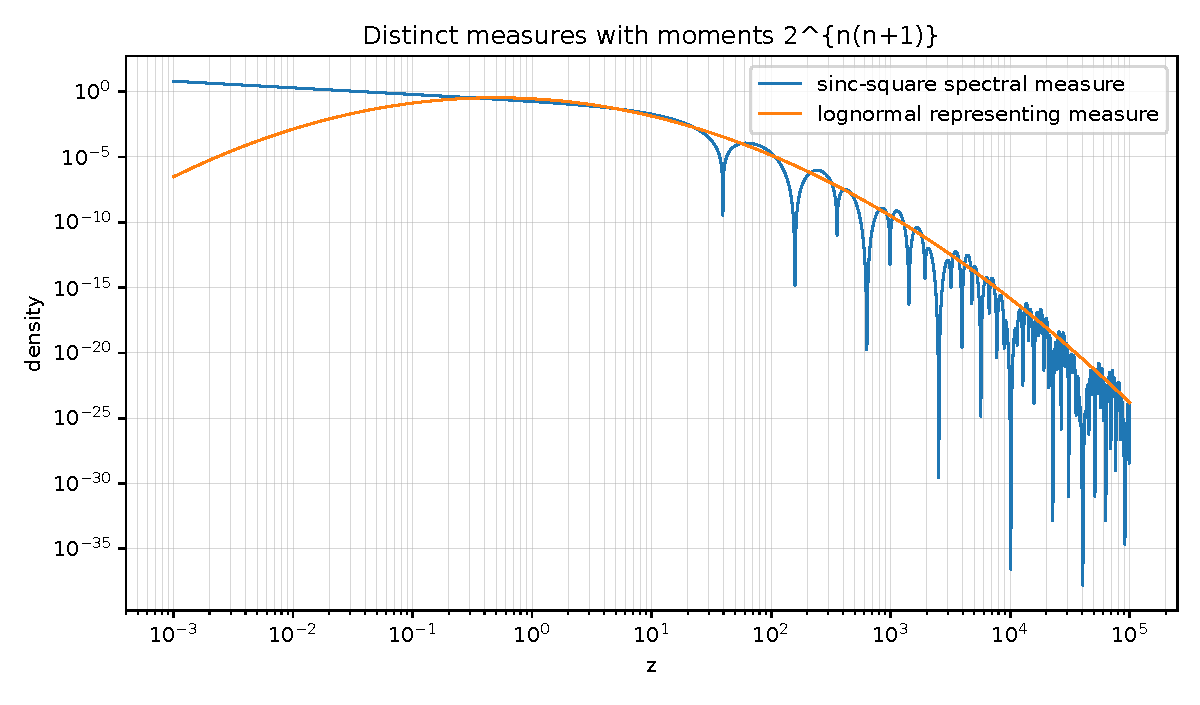
\includegraphics[width=0.91\textwidth]{spectral_vs_lognormal.pdf}
\caption{The sinc-square spectral density and a lognormal density have exactly the same
nonnegative integer moments but visibly different local structures.  The spectral zeros are
inherited from the integer zeros of the infinite sinc product.}
\label{fig:spectral-vs-lognormal}
\end{figure}

\subsection{A nonclassical q-Pearson equation}

The Fourier product satisfies
\begin{equation}
 \Phi(2\xi)=\sinc(2\pi\xi)\Phi(\xi).
 \label{eq:Phi-scaling}
\end{equation}

\begin{proposition}[Sinc-square q-Pearson law]
\label{prop:q-Pearson}
The spectral density \eqref{eq:spectral-density} obeys
\begin{equation}
 \boxed{
 w_{\rm sp}(4z)=\frac12\sinc^2(\sqrt z)\,w_{\rm sp}(z).}
 \label{eq:spectral-q-Pearson}
\end{equation}
By contrast, the lognormal representative satisfies
\begin{equation}
 w_{\rm ln}(4z)=\frac1{4z}w_{\rm ln}(z).
 \label{eq:lognormal-q-Pearson}
\end{equation}
\end{proposition}

\begin{proof}
In \eqref{eq:spectral-density}, replacing $z$ by $4z$ doubles the Fourier argument and
multiplies the square-root denominator by $2$.  Apply \eqref{eq:Phi-scaling} and note that
$2\pi(\sqrt z/(2\pi))=\sqrt z$.  The lognormal identity follows by direct substitution in
\eqref{eq:lognormal-density}.
\end{proof}

\begin{remark}
Classical Stieltjes--Wigert measures satisfy q-Pearson equations with monomial or rational
multipliers.  Equation \eqref{eq:spectral-q-Pearson} replaces that multiplier by an entire
sinc-square factor carrying the complete integer-zero divisor.  Determining its position in
the Nevanlinna family is one of the principal open directions in \Cref{sec:future}.
\end{remark}

\section{Hankel determinants, q-binomial polynomials, and Lagrange quadrature}
\label{sec:q-orthogonal}

Fix $0<q<1$ and the moment sequence
\begin{equation}
 m_n=q^{-n(n+1)/2}.
 \label{eq:general-q-moments}
\end{equation}
The Fabius--Rvachev spectral case is $q=1/4$.

\begin{theorem}[Hankel determinants]
\label{thm:Hankel-determinants}
For $N\geq0$,
\begin{equation}
 \boxed{
 \Delta_N:=\det[m_{i+j}]_{i,j=0}^{N}
 =q^{-N(N+1)(4N+5)/6}
 \prod_{k=1}^{N}(q;q)_k,}
 \label{eq:Hankel-determinant}
\end{equation}
where $(q;q)_k=\prod_{r=1}^k(1-q^r)$.
\end{theorem}

\begin{proof}
Factor
\[
 m_{i+j}=q^{-i(i+1)/2}q^{-j(j+1)/2}q^{-ij}.
\]
The row and column factors contribute
$q^{-\sum_{i=0}^N i(i+1)}$.  The remaining determinant is the Vandermonde determinant in
$q^{-i}$:
\[
 \det[(q^{-i})^j]_{i,j=0}^N
 =\prod_{0\leq i<k\leq N}(q^{-k}-q^{-i})
 =q^{-\sum_{k=1}^Nk^2}\prod_{k=1}^{N}(q;q)_k.
\]
Finally
\[
 \sum_{i=1}^{N}i(i+1)+\sum_{i=1}^{N}i^2
 =\frac{N(N+1)(4N+5)}6.
\]
\end{proof}

\begin{theorem}[Monic shifted Stieltjes--Wigert polynomials]
\label{thm:SW-polynomials}
The monic orthogonal polynomial of degree $n$ for any representing measure of
\eqref{eq:general-q-moments} is
\begin{equation}
 \boxed{
 P_n(z)=\sum_{k=0}^{n}
 (-1)^{n-k}q^{k^2-n^2}\qbinom{n}{k}{q}\,z^k.}
 \label{eq:SW-polynomial}
\end{equation}
It satisfies
\begin{equation}
 \int z^jP_n(z)\dd\mu(z)=0,
 \qquad0\leq j<n,
 \label{eq:SW-orthogonality}
\end{equation}
for every measure $\mu$ with moments \eqref{eq:general-q-moments}, and
\begin{equation}
 h_n:=\int P_n(z)^2\dd\mu(z)
 =q^{-(2n^2+n)}(q;q)_n.
 \label{eq:SW-norm}
\end{equation}
The three-term recurrence is
\begin{equation}
 P_{n+1}(z)=(z-a_n)P_n(z)-b_nP_{n-1}(z),
 \label{eq:SW-recurrence}
\end{equation}
with
\begin{align}
 a_n&=q^{-2n-1}(1+q-q^{n+1}),\label{eq:an}\\
 b_n&=q^{-(4n-1)}(1-q^n),\qquad n\geq1.
 \label{eq:bn}
\end{align}
\end{theorem}

\begin{proof}
Let $c_k$ be the coefficient of $z^k$ in \eqref{eq:SW-polynomial}.  For $j<n$,
\begin{align*}
 \sum_{k=0}^{n}c_km_{k+j}
 &=(-1)^nq^{-n^2-j(j+1)/2}
 \sum_{k=0}^{n}(-1)^kq^{k(k-1)/2}
 \qbinom{n}{k}{q}q^{-jk}\\
 &=(-1)^nq^{-n^2-j(j+1)/2}(q^{-j};q)_n=0,
\end{align*}
by the finite q-binomial theorem; one factor is $1-q^0$.  The leading coefficient is one.
The norm is the standard Gram-determinant quotient
$h_n=\Delta_n/\Delta_{n-1}$, which gives \eqref{eq:SW-norm}.  Hence
$b_n=h_n/h_{n-1}$.  Comparing the coefficients of $z^n$ in the monic recurrence gives
$a_n$; the coefficient of $z^{n-1}$ in $P_n$ is
$-q^{-2n+1}(1-q^n)/(1-q)$, yielding \eqref{eq:an}.
\end{proof}

For $q=1/4$, the first polynomials are
\begin{align}
 P_0(z)&=1,\nonumber\\
 P_1(z)&=z-4,\nonumber\\
 P_2(z)&=z^2-80z+256,\nonumber\\
 P_3(z)&=(z-64)(z^2-1280z+4096).
 \label{eq:first-SW-polynomials}
\end{align}

\subsection{Gaussian quadrature as q-binomial Lagrange interpolation}

Let $\lambda_{n,1},\ldots,\lambda_{n,n}$ be the zeros of $P_n$ and let
$\ell_{n,j}$ be the Lagrange cardinal polynomial at these nodes.  The Gaussian weights are
\begin{equation}
 \omega_{n,j}:=\int\ell_{n,j}(z)\dd\mu(z)
 =\left(\sum_{r=0}^{n-1}\frac{P_r(\lambda_{n,j})^2}{h_r}\right)^{-1}.
 \label{eq:Christoffel-weights}
\end{equation}
Because the polynomials and $h_r$ are determined by the moment sequence, the nodes and
weights are identical for $\mu_{\rm sp}$, the lognormal measure, and every other representing
measure.

\begin{corollary}[Measure-independent Gaussian quadrature]
\label{cor:Gaussian-quadrature}
For every polynomial $Q$ of degree at most $2n-1$,
\begin{equation}
 \boxed{
 \int_0^\infty Q(z)\dd\mu_{\rm sp}(z)
 =\sum_{j=1}^{n}\omega_{n,j}Q(\lambda_{n,j})
 =\int_0^\infty Q(z)w_{\rm ln}(z)\dd z.}
 \label{eq:Gaussian-quadrature}
\end{equation}
The q-binomial coefficients in \eqref{eq:SW-polynomial} therefore generate exact finite
Lagrange quadrature rules for polynomial spectral energies of the infinite sinc product.
\end{corollary}

\begin{remark}
Moment indeterminacy is invisible to every finite polynomial test: all representing measures
produce the same Gaussian quadrature.  The distinction lives in the orthogonal complement of
the polynomial closure, exactly where the integer-zero geometry of $\Phi$ can enter.
\end{remark}

\section{The optimal derivative weight and a q-Legendre Fourier envelope}
\label{sec:carleman}

\subsection{Exact Denjoy--Carleman weight}

Define
\begin{equation}
 M_n:=2^{T_n}=2^{n(n+1)/2}.
 \label{eq:Mn}
\end{equation}
By \eqref{eq:Linf-exact}, $\Up$ saturates this derivative weight exactly:
\begin{equation}
 \norm{\Up^{(n)}}_\infty=M_n.
 \label{eq:saturates-Mn}
\end{equation}
The sequence is logarithmically convex and
\begin{equation}
 \frac{M_n}{M_{n+1}}=2^{-(n+1)},
 \qquad
 \sum_{n=0}^{\infty}\frac{M_n}{M_{n+1}}=1<\infty.
 \label{eq:nonquasianalytic-sum}
\end{equation}
Thus the direct-weight Denjoy--Carleman class generated by $M$ is nonquasianalytic, as the
existence of the compactly supported nonzero function $\Up$ requires.

\begin{proposition}[Outside every finite Gevrey class]
\label{prop:not-Gevrey}
For no finite $s>0$ do constants $A,C>0$ satisfy
\begin{equation}
 M_n\leq CA^n(n!)^s\qquad(n\geq0).
 \label{eq:no-Gevrey-bound}
\end{equation}
Hence $\Up$ belongs to no finite-order Gevrey class on any interval containing its support.
\end{proposition}

\begin{proof}
The logarithm of $M_n$ is $(\log2)n^2/2+\bigO(n)$, whereas
$\log((n!)^sA^n)=sn\log n+\bigO(n)$.  The quadratic term wins.
\end{proof}

\subsection{Exact associated function and periodic lattice correction}

Define the associated function
\begin{equation}
 \omega_M(t):=\sup_{n\geq0}\log\frac{t^n}{M_n},
 \qquad t>0.
 \label{eq:associated-function}
\end{equation}
Let $r=\log_2t$.

\begin{theorem}[Exact q-Legendre transform]
\label{thm:q-Legendre}
For $r\geq1/2$,
\begin{equation}
 \boxed{
 \omega_M(t)=\frac{\log2}{2}
 \left[
 \left(r-\frac12\right)^2
 -\dist\!\left(r-\frac12,\N_0\right)^2
 \right].}
 \label{eq:q-Legendre}
\end{equation}
For $r\leq1/2$, $\omega_M(t)=0$.  Thus the continuous log-square Legendre transform carries
an exact bounded one-periodic lattice correction in $\log_2t$.
\end{theorem}

\begin{proof}
For each integer $n\geq0$,
\[
 \log\frac{t^n}{M_n}
 =\log2\left(nr-\frac{n(n+1)}2\right)
 =\frac{\log2}{2}\left[
 \left(r-\frac12\right)^2-
 \left(n-r+\frac12\right)^2\right].
\]
Maximizing means choosing the nearest nonnegative integer to $r-1/2$.  If $r\leq1/2$, the
maximum is attained at $n=0$ and equals zero.
\end{proof}

\begin{corollary}[Optimized integration-by-parts envelope]
\label{cor:IBP-envelope}
For every $\xi\neq0$,
\begin{equation}
 \boxed{
 |\Phi(\xi)|
 \leq\inf_{n\geq0}\frac{M_n}{(2\pi|\xi|)^n}
 =\exp\bigl(-\omega_M(2\pi|\xi|)\bigr).}
 \label{eq:IBP-envelope}
\end{equation}
If $r=\log_2(2\pi|\xi|)\geq1/2$, this is
\begin{equation}
 |\Phi(\xi)|\leq
 2^{-\frac12(r-1/2)^2+\frac12\dist(r-1/2,\N_0)^2}.
 \label{eq:explicit-IBP-envelope}
\end{equation}
\end{corollary}

\begin{proof}
Integrating the Fourier transform by parts $n$ times and using
\eqref{eq:L1-exact} gives
$|\Phi(\xi)|\leq M_n/(2\pi|\xi|)^n$.  Optimize with
\Cref{thm:q-Legendre}.
\end{proof}

\begin{warning}
The envelope \eqref{eq:explicit-IBP-envelope} is the best one obtainable from the exact
$L^1$ derivative norms alone; it is not the sharp pointwise or annular Fourier envelope.
The Fourier-decay reports in the corpus exploit the lacunary sine cocycle and obtain stronger
linear-in-$\log|\xi|$ corrections.  The value of \eqref{eq:explicit-IBP-envelope} is its exact
functional-analytic duality with the derivative weight, not a replacement for those sharper
results.
\end{warning}

\section{Numerical experiments}
\label{sec:numerics}

All code used here is in \texttt{numerical\_experiments.py}.  It is included with detailed
comments in the accompanying archive.  The script reconstructs $\Up$ by inverse FFT on a
periodic box of length $4$ from $55$ dyadic sinc factors, using $2^{19}$ samples.  Since
$\Up$ is supported on $[-1,1]$, the box supplies exact geometric zero padding.  The run used
\[
 \Delta x=2^{-17}=7.62939453125\times10^{-6},
 \qquad \Delta\xi=\frac14.
\]
The reconstructed density had integral $1$ and value $\Up(0)=1$ to displayed precision;
the largest value outside the support was $3.33\times10^{-16}$.

\subsection{Derivative tiling and norm checks}

\begin{figure}[htbp]
\centering
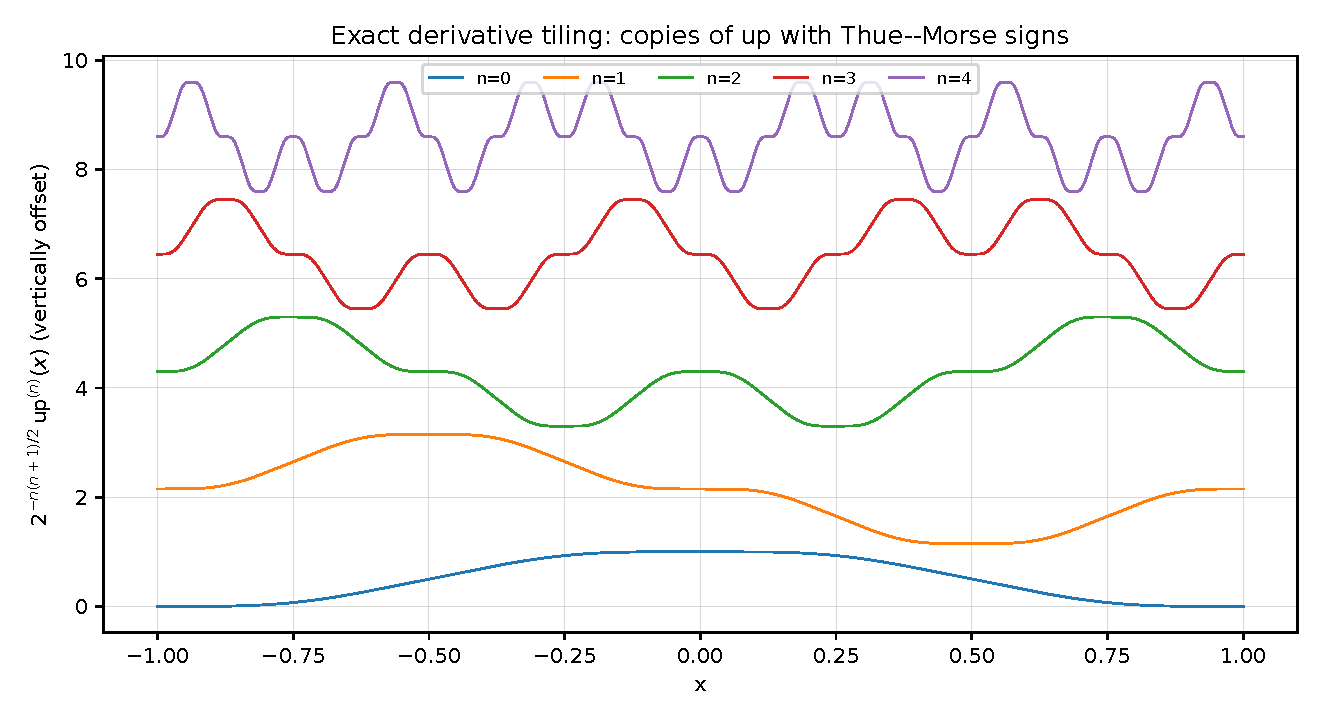
\includegraphics[width=0.94\textwidth]{derivative_tiling.pdf}
\caption{Normalized derivatives $2^{-T_n}\Up^{(n)}$, vertically offset.  Each row is a
concatenation of copies of the original bump; their signs are the length-$2^n$ Thue--Morse
block.}
\label{fig:derivative-tiling}
\end{figure}

For $n=0,\ldots,6$ and $p\in\{1,2,4,8,\infty\}$, the script formed the derivative from the
exact cell formula and compared its numerical norm with
$2^{T_n}\norm{\Up}_p$.  The largest absolute deviation of the ratio from $1$ was
$2.22\times10^{-16}$.

\subsection{Spectral moments}

\begin{center}
\small
\begin{tabular}{@{}rrrr@{}}
\toprule
$n$ & numerical $\int(2\pi\xi)^{2n}|\Phi|^2$ & predicted $2^{n(n+1)}C_2$ & relative error\\
\midrule
0 & $8.088735359679706\times10^{-1}$ & $8.088735359679707\times10^{-1}$ & $-1.11\times10^{-16}$\\
1 & $3.235494143871882$ & $3.235494143871883$ & $-2.22\times10^{-16}$\\
2 & $5.176790630195011\times10^{1}$ & $5.176790630195013\times10^{1}$ & $-2.22\times10^{-16}$\\
3 & $3.313146003324810\times10^{3}$ & $3.313146003324808\times10^{3}$ & $4.44\times10^{-16}$\\
4 & $8.481653768511517\times10^{5}$ & $8.481653768511509\times10^{5}$ & $8.88\times10^{-16}$\\
5 & $8.685213458955796\times10^{8}$ & $8.685213458955785\times10^{8}$ & $1.33\times10^{-15}$\\
6 & $3.557463432788293\times10^{12}$ & $3.557463432788290\times10^{12}$ & $8.88\times10^{-16}$\\
7 & $5.828548088280333\times10^{16}$ & $5.828548088280334\times10^{16}$ & $-1.11\times10^{-16}$\\
\bottomrule
\end{tabular}
\end{center}

The near-machine equality is a stringent joint check of the FFT normalization, derivative
scale, Parseval convention, and moment exponent.

\subsection{Euler--Gamma operator convergence}

The inverse interpolant was obtained directly from
$G(1-\Up(x))=x$ on $0\leq x\leq1$.  Logarithmic finite differences estimated
$\Dop^kG(1/p)$ for $k\leq3$.  The following table lists relative errors of successive
truncations of \eqref{eq:Gamma-operator-first-terms}.

\begin{center}
\small
\begin{tabular}{@{}rrrrrr@{}}
\toprule
$p$ & $A_p/G(1/p)$ & $G$ only & through $\Dop$ & through $\Dop^2$ & through $\Dop^3$\\
\midrule
256   & 0.92618125 & $-7.38\!\times10^{-2}$ & $4.84\!\times10^{-2}$ & $-1.47\!\times10^{-2}$ & $6.46\!\times10^{-3}$\\
512   & 0.92793214 & $-7.21\!\times10^{-2}$ & $4.32\!\times10^{-2}$ & $-1.20\!\times10^{-2}$ & $6.37\!\times10^{-3}$\\
1024  & 0.92942377 & $-7.06\!\times10^{-2}$ & $3.91\!\times10^{-2}$ & $-9.78\!\times10^{-3}$ & $4.87\!\times10^{-3}$\\
2048  & 0.93089393 & $-6.91\!\times10^{-2}$ & $3.60\!\times10^{-2}$ & $-8.37\!\times10^{-3}$ & $3.35\!\times10^{-3}$\\
4096  & 0.93235311 & $-6.76\!\times10^{-2}$ & $3.33\!\times10^{-2}$ & $-7.55\!\times10^{-3}$ & $2.53\!\times10^{-3}$\\
8192  & 0.93370939 & $-6.63\!\times10^{-2}$ & $3.09\!\times10^{-2}$ & $-6.86\!\times10^{-3}$ & $2.39\!\times10^{-3}$\\
16384 & 0.93492704 & $-6.51\!\times10^{-2}$ & $2.87\!\times10^{-2}$ & $-6.10\!\times10^{-3}$ & $2.29\!\times10^{-3}$\\
32768 & 0.93604971 & $-6.40\!\times10^{-2}$ & $2.69\!\times10^{-2}$ & $-5.39\!\times10^{-3}$ & $1.97\!\times10^{-3}$\\
65536 & 0.93712995 & $-6.29\!\times10^{-2}$ & $2.53\!\times10^{-2}$ & $-4.83\!\times10^{-3}$ & $1.60\!\times10^{-3}$\\
\bottomrule
\end{tabular}
\end{center}

\begin{figure}[htbp]
\centering
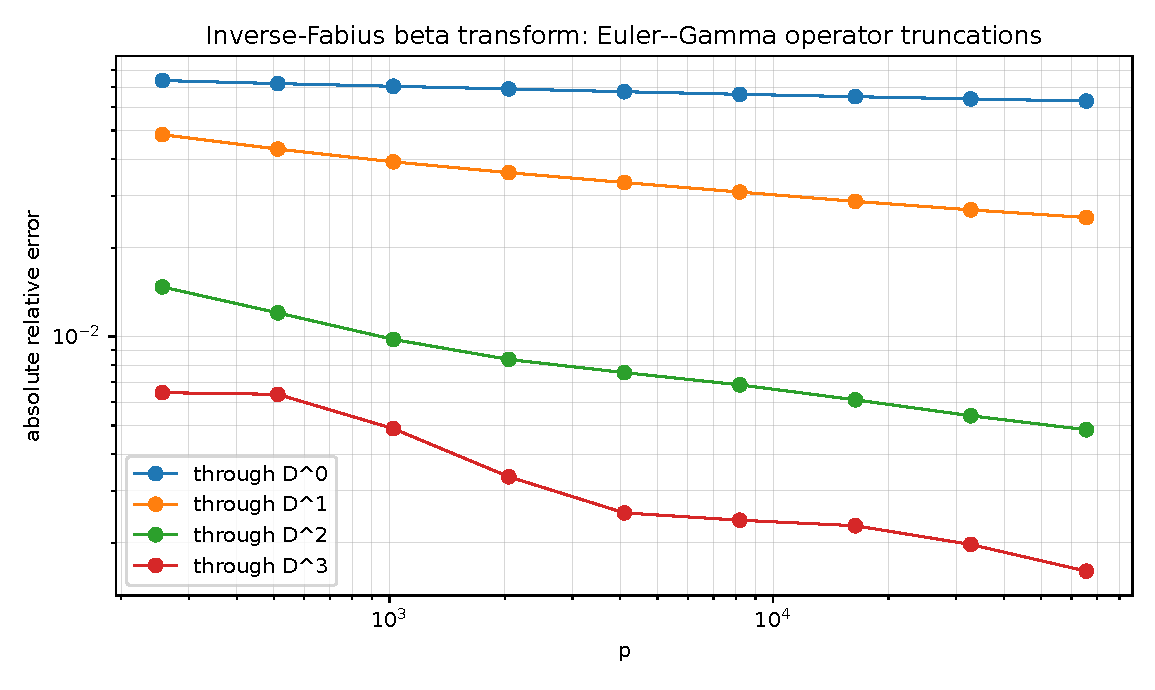
\includegraphics[width=0.87\textwidth]{beta_operator_errors.pdf}
\caption{Absolute relative errors of the first four Euler--Gamma operator truncations.  The
slow scale $\rho^{-1}\asymp(\log p)^{-1/2}$ explains why very large $p$ is needed before
successive asymptotic orders separate cleanly.}
\label{fig:beta-errors}
\end{figure}

\subsection{Symbolic Hankel checks}

SymPy evaluated the determinants in \eqref{eq:Hankel-determinant} exactly for
$N=0,\ldots,6$ at $q=1/4$; every quotient of the direct determinant by the claimed closed
form simplified to $1$.  The base-$10$ logarithms of the determinants for $N=1,\ldots,6$
were
\[
 1.68124,\ 7.54887,\ 20.03233,\ 41.54498,\ 74.49635,\ 121.29499,
\]
illustrating the rapid $q^{-\frac23N^3+\bigO(N^2)}$ growth.

\section{Conjectures and promising research directions}
\label{sec:future}

\subsection{A full norm transseries}

The inverse report gives an all-orders expansion of $G$ in the differential algebra generated
by periodic saddle jets.  The exact operator \eqref{eq:exact-operator} should transport that
algebra to the norm spectrum without introducing any new transcendental data beyond the
log-exponential cumulants.

\begin{conjecture}[All-orders Gamma--Lambert norm transseries]
\label{conj:full-norm-transseries}
There exist one-periodic real-analytic coefficient functions
$C_{m,\ell}(\theta)$ such that
\begin{equation}
 \frac{\norm{\Up}_p^p}{2G_0(p^{-1})}
 \sim1+\sum_{m=1}^{\infty}\rho^{-m}
 \sum_{\ell=0}^{m}C_{m,\ell}(\theta)(\log\rho)^\ell,
 \label{eq:full-norm-transseries}
\end{equation}
with $C_{1,1}=1/2$ and
$C_{1,0}=\kappa_0-\gamma-\Psi(\theta)$.  Every $C_{m,\ell}$ belongs to the differential
algebra generated by the inverse saddle jets and the constants
$\gamma,\zeta(2),\ldots,\zeta(m)$; no additional periodic functions occur.
\end{conjecture}

A proof should combine the formal inverse recursion already in the corpus with a tame
remainder theorem for the operator $M_p(\Dop)$.  The key analytic task is uniform control of
$\Dop^mG$ on logarithmic windows whose width grows slowly with $\rho$.

\subsection{Nevanlinna parameter of the sinc-square measure}

\begin{problem}[Locate $\mu_{\rm sp}$ in the Stieltjes--Wigert Nevanlinna family]
\label{prob:Nevanlinna}
Determine the Nevanlinna parameter corresponding to the density
\eqref{eq:spectral-density}.  Equivalently, calculate the Cauchy transform
\begin{equation}
 S_{\rm sp}(z)=\int_0^\infty\frac{\dd\mu_{\rm sp}(t)}{z-t}
 \label{eq:spectral-Stieltjes-transform}
\end{equation}
relative to the classical entire functions $A,B,C,D$ of the shifted
Stieltjes--Wigert moment problem.
\end{problem}

The exact q-Pearson law \eqref{eq:spectral-q-Pearson} supplies unusually rigid extra data.
One promising route is to Mellin-transform it, obtaining a functional equation coupling the
spectral Mellin transform to the Mellin transform of $\sinc^2(\sqrt z)$.  Another is to use
the canonical product of $\Phi$ to express $S_{\rm sp}$ as a convergent sum over integer-zero
lobes.

\begin{conjecture}[Sinc-Pearson uniqueness]
\label{conj:sinc-Pearson-uniqueness}
Among absolutely continuous representing measures of
$m_n=2^{n(n+1)}$ whose density is locally bounded after multiplication by $\sqrt z$, the
normalization, moment conditions, and q-Pearson equation
\eqref{eq:spectral-q-Pearson} determine $w_{\rm sp}$ uniquely.
\end{conjecture}

\subsection{Orthogonal complement and spectral zeros}

For an indeterminate moment problem, the polynomials are not dense in every representing
$L^2$ space.  The spectral measure should possess an orthogonal complement reflecting the
integer-zero structure of $\Phi$.

\begin{problem}[Explicit nonpolynomial orthogonal basis]
Construct functions $Q_j(z)$ such that
\[
 \int_0^\infty z^nQ_j(z)w_{\rm sp}(z)\dd z=0
 \qquad(n\geq0)
\]
and such that the $Q_j$ span the orthogonal complement of the shifted
Stieltjes--Wigert polynomials in $L^2(\mu_{\rm sp})$.  Dyadic rescalings of sinc factors,
integer-lobe indicator functions, and q-Bessel functions from the classical theory are the
three natural candidate families.
\end{problem}

\subsection{Confluent q-Richardson phase tomography}

The existing corpus develops Gaussian-q Richardson weights for pure power error germs.
The norm expansion \eqref{eq:full-norm-transseries} contains powers multiplied by logarithms.
Choose a fixed phase $\vartheta$ and a dyadic phase-locked sequence
\begin{equation}
 \rho_j=M2^j+\delta,
 \qquad
 \delta+\beta\equiv\vartheta\pmod1,
 \qquad
 p_j=\exp(L\rho_j^2/2).
 \label{eq:dyadic-phase-nodes}
\end{equation}
Then $h_j=1/\rho_j$ is an analytic function of $2^{-j}$, while the phase is constant.
After subtracting the known logarithmic terms, the remaining errors are combinations of
$j^\ell2^{-mj}$.

\begin{conjecture}[Confluent Gaussian-q filter]
\label{conj:confluent-q-filter}
For each truncation order $r$, there is a stable finite filter whose shift polynomial is a
product of repeated factors
\begin{equation}
 \prod_{m=1}^{r}(E-2^{-m})^{d_m},
 \label{eq:confluent-shift-polynomial}
\end{equation}
which annihilates every error mode $j^\ell2^{-mj}$ with
$0\leq\ell<d_m$.  Its coefficients can be written as derivatives or confluent limits of the
Gaussian-q-binomial Lagrange weights
\begin{equation}
 w_{r,j}(q)=(-1)^{r-j}
 \frac{q^{\binom{r-j+1}{2}}}{(q;q)_j(q;q)_{r-j}}.
 \label{eq:q-Richardson-weights}
\end{equation}
Applied to \eqref{eq:dyadic-phase-nodes}, this filter recovers
$\kappa_0-\gamma-\Psi(\vartheta)$ with a rigorously controlled error of arbitrarily high
order in $2^{-j}$.
\end{conjecture}

This would create a genuinely new Richardson pipeline: the data are global derivative norms,
the target is a pointwise endpoint periodic function, and the logarithmic multiplicities are
handled by confluent q-Lagrange interpolation.

\subsection{Base-b and Pascal--Rvachev extensions}

The Pascal--Rvachev hierarchy in the corpus replaces the single sinc exponent by binomial
multiplicities.  The present analysis suggests two extensions.

\begin{problem}[Norm ladders for higher Rvachev ranks]
For each hierarchy level, identify a spatial refinement formula with disjoint or finitely
overlapping cells, determine whether normalized derivatives are equimeasurable with a fixed
profile, and calculate the resulting derivative weight.  If exact equimeasurability fails,
seek a finite-state transfer operator for value distributions.
\end{problem}

\begin{conjecture}[Higher-rank lognormal moment geometry]
For the rank-$r$ Pascal--Rvachev profile, the normalized spectral energy moments are
$q$-hyperfactorial sequences whose Hankel determinants factor into products of
$q$-Pochhammer symbols with exponents polynomial in the index.  The associated orthogonal
polynomials should be multilevel q-binomial deformations of Stieltjes--Wigert polynomials.
\end{conjecture}

\subsection{Formalization roadmap}

The roadmap is now partly discharged.  The completion labels below refer only to the named
declarations in \path{RvachevDerivativeDistribution.lean}; they do not mark the whole report
as formalized.  A practical order is:
\begin{enumerate}
\item \textbf{Completed.}  The derivative tiling has a public exact cell coordinate,
      endpoint/range lemmas, signed and absolute cellwise formulas, and signed midpoint
      corollary.
\item \textbf{Absolute part completed.}  The normalized absolute law is an exact Borel
      pushforward equality and has Banach-valued continuous-test forms.  The signed
      finite-mixture identity is also formal for continuous Banach-valued tests and all
      \(n\), but its simplified signed Rademacher Borel law remains open.
\item \textbf{Still open beyond completed prerequisites.}  Use the all-\(p\ge0\)
      real-power moment theorem, midpoint signs, and existing pointwise bounds to derive
      \path{eLpNorm}, general rearrangement-invariant, total-variation, and exact
      inverse-Fabius level-set corollaries.
\item \textbf{Open.}  Formalize the Stieltjes substitution and beta-transform identity for
      the totalized inverse.
\item \textbf{Open.}  Prove the spectral moments by the existing Fourier differentiation
      API.
\item \textbf{Open.}  Formalize the Vandermonde determinant and finite q-binomial
      orthogonality.
\item \textbf{Deferred.}  Treat the all-orders asymptotic operator after the inverse
      derivative-jet bounds have a stable public interface.
\end{enumerate}

\section{Conclusion}

The dyadic derivative formula contains more information than its usual pointwise reading
suggests.  Because the cells are disjoint and all have the same affine Jacobian, it is an
exact renormalization fixed point for value distributions.  The entire derivative tower has
one absolute profile, amplified by $2^{n(n+1)/2}$ and signed by Thue--Morse.  This immediately
produces an exact norm spectrum in every rearrangement-invariant space and makes the inverse
Fabius function the level-set law of every derivative.

Two dual transforms then emerge.  In physical space, the large-$p$ norms are a beta average
of the inverse function.  The beta dilation converges to an exponential dilation, whose
Mellin symbol is $\Gamma(1+s)$; Bell polynomials, zeta values, and Bernoulli polynomials are
therefore forced into the asymptotic operator.  Combining it with the lower-Lambert endpoint
coordinate reveals a universal Euler-constant shift and lets global norms perform phase
tomography on the periodic saddle correction.

In frequency space, Parseval turns the same derivative scale into the moment sequence
$2^{n(n+1)}$.  The infinite sinc product thus supplies an explicit, highly nonclassical
Stieltjes--Wigert representing measure.  Its integer zeros distinguish it from the lognormal
representative even though all polynomial moments agree; its q-Pearson law retains the full
sinc-square factor.  The resulting q-binomial orthogonal polynomials and Gaussian Lagrange
rules give a concrete bridge between spectral energy, moment indeterminacy, and the
$q$-calculus already pervasive in the Fabius theory.

The most promising analytic next step is to identify the sinc-square measure inside the
Nevanlinna family.  On the formal side, the dyadic-cell and normalized absolute
equimeasurability core is now complete.  The next compact targets are its
\path{eLpNorm}/rearrangement-invariant and inverse-Fabius level-set consequences, followed
by the beta-transform layer.  The signed Rademacher Borel simplification and every
beta/spectral layer in this report remain frontier statements.

\appendix

\section{Recursive TeX corpus ledger}
\label{app:corpus-ledger}

The following $68$ paths were present under
\path{Analysis/FabiusFunction/docs} at commit \RepoCommit.  Archived versions were included
in the collision audit but interpreted according to the archive's provenance ledger.

\begingroup
\small
\renewcommand{\arraystretch}{1.08}
\begin{longtable}{@{}r>{\raggedright\arraybackslash}p{0.88\textwidth}@{}}
\toprule
\# & Path\\
\midrule
\endfirsthead
\toprule
\# & Path (continued)\\
\midrule
\endhead
1 & \path{FabiusFunction_Mathematical_Glossary/FabiusFunction_Mathematical_Glossary.tex}\\
2 & \path{Fabius_Function_and_Rvachev_Up/Fabius_Function_and_Rvachev_Up.tex}\\
3 & \path{Non_Elementarity_of_the_Fabius_Function/Non_Elementarity_of_the_Fabius_Function.tex}\\
4 & \path{archive/early-notes/Fabius Asymptotic/Fabius Asymptotic.tex}\\
5 & \path{archive/early-notes/K-fold summation over the signed Thue-Morse sequence/K-fold summation over the signed Thue-Morse sequence.tex}\\
6 & \path{archive/glossary/FabiusFunction_Mathematical_Glossary-2/FabiusFunction_Mathematical_Glossary.tex}\\
7 & \path{archive/glossary/FabiusFunction_Mathematical_Glossary/FabiusFunction_Mathematical_Glossary.tex}\\
8 & \path{archive/lean-walkthrough/Fabius_Function_Lean_Walkthrough/Fabius_Function_Lean_Walkthrough.tex}\\
9 & \path{archive/lean-walkthrough/fabius_lean_walkthrough/fabius_lean_walkthrough.tex}\\
10 & \path{archive/primary-exposition/Fabius_Function_and_Rvachev_Up-2/Fabius_Function_and_Rvachev_Up.tex}\\
11 & \path{archive/primary-exposition/Fabius_Function_and_Rvachev_Up-3/Fabius_Function_and_Rvachev_Up.tex}\\
12 & \path{archive/primary-exposition/Fabius_Function_and_Rvachev_Up/Fabius_Function_and_Rvachev_Up.tex}\\
13 & \path{archive/primary-exposition/Fabius_and_Rvachev_Up-2/Fabius_and_Rvachev_Up.tex}\\
14 & \path{archive/primary-exposition/Fabius_and_Rvachev_up/Fabius_and_Rvachev_up.tex}\\
15 & \path{archive/primary-exposition/Fabius_function_and_up_function/Fabius_function_and_up_function.tex}\\
16 & \path{archive/primary-supplements/Fabius_Function_Missing_Parts-2/Fabius_Function_Missing_Parts.tex}\\
17 & \path{archive/primary-supplements/Fabius_Function_Missing_Parts/Fabius_Function_Missing_Parts.tex}\\
18 & \path{archive/q-calculus/Fabius_q_Special_Functions/Fabius_q_Special_Functions.tex}\\
19 & \path{archive/q-calculus/fabius-q-special-functions/fabius-q-special-functions.tex}\\
20 & \path{archive/research-frontiers/Fabius_Dyadic_Asymptotic_Bridge/Fabius_Dyadic_Asymptotic_Bridge.tex}\\
21 & \path{archive/research-frontiers/Fabius_Dyadic_Formulae_and_Alternative_Representations/Fabius_Dyadic_Formulae_and_Alternative_Representations.tex}\\
22 & \path{archive/research-frontiers/Fabius_Dyadic_Formulae_to_Asymptotics/Fabius_Dyadic_Formulae_to_Asymptotics.tex}\\
23 & \path{archive/research-frontiers/Fabius_Dyadic_q_Connections/Fabius_Dyadic_q_Connections.tex}\\
24 & \path{archive/research-frontiers/Fabius_Thue_Morse_Convergence_Rate/Fabius_Thue_Morse_Convergence_Rate.tex}\\
25 & \path{archive/research-frontiers/Fabius_Thue_Morse_Convergence_Rates/Fabius_Thue_Morse_Convergence_Rates.tex}\\
26 & \path{archive/research-frontiers/Primary_Exposition_Gap_Register/Primary_Exposition_Gap_Register.tex}\\
27 & \path{archive/research-frontiers/Repeated_Integration_and_Rvachev_Up/Repeated_Integration_and_Rvachev_Up.tex}\\
28 & \path{archive/research-frontiers/Rvachev_Up_from_Repeated_Integration/Rvachev_Up_from_Repeated_Integration.tex}\\
29 & \path{archive/research-frontiers/Thue_Morse_Formula_Atlas-1/Thue_Morse_Formula_Atlas.tex}\\
30 & \path{archive/research-frontiers/Thue_Morse_Formula_Atlas-2/Consolidated_Formula_Atlas_for_the_Thue_Morse_Sequence.tex}\\
31 & \path{archive/research-frontiers/Thue_Morse_Formula_Atlas-3/Thue_Morse_Formula_Atlas.tex}\\
32 & \path{archive/research-frontiers/non-formalized-research-frontiers/non-formalized-research-frontiers.tex}\\
33 & \path{archive/standalone-studies/Non_Elementarity_of_the_Fabius_Function/Non_Elementarity_of_the_Fabius_Function.tex}\\
34 & \path{archive/standalone-studies/Small_Argument_Asymptotics/Small_Argument_Asymptotics.tex}\\
35 & \path{archive/standalone-studies/fabius-inverse-dyadic-closed-form/fabius-inverse-dyadic-closed-form.tex}\\
36 & \path{fabius_lean_walkthrough/fabius_lean_walkthrough.tex}\\
37 & \path{non-formalized-research-frontiers/non-formalized-research-frontiers.tex}\\
38 & \path{non-formalized-research-frontiers/drafts/Fabius_Arithmetic_Rays_Frontier_Report/Fabius_Arithmetic_Rays_Frontier_Report.tex}\\
39 & \path{non-formalized-research-frontiers/drafts/Fabius_Half_Integer_Spectral_Frontier_Report/Fabius_Half_Integer_Spectral_Frontier_Report.tex}\\
40 & \path{non-formalized-research-frontiers/drafts/Fabius_Inverse_Frontier_Report_Source_and_PDF/Fabius_Inverse_Frontier_Report.tex}\\
41 & \path{non-formalized-research-frontiers/drafts/Fabius_Rvachev_Frontier_Report-2/Fabius_Rvachev_Frontier_Report.tex}\\
42 & \path{non-formalized-research-frontiers/drafts/Fabius_Rvachev_Frontier_Report/Fabius_Rvachev_Frontier_Report.tex}\\
43 & \path{non-formalized-research-frontiers/drafts/Fabius_Rvachev_New_Frontiers/Fabius_Rvachev_New_Frontiers.tex}\\
44 & \path{non-formalized-research-frontiers/drafts/Fabius_Rvachev_Thue_Morse_Frontier_Results/Fabius_Rvachev_Thue_Morse_Frontier_Results.tex}\\
45 & \path{non-formalized-research-frontiers/drafts/Spectral_Arithmetic_Pascal_Rvachev_Hierarchy/Spectral_Arithmetic_Pascal_Rvachev_Hierarchy.tex}\\
46 & \path{non-formalized-research-frontiers/drafts/Thue_Morse_Formula_Atlas/Thue_Morse_Formula_Atlas.tex}\\
47 & \path{non-formalized-research-frontiers/drafts/fabius_frontier_new_results/fabius_frontier_new_results.tex}\\
48 & \path{non-formalized-research-frontiers/drafts/fabius_frontier_results_bundle/fabius_frontier_results.tex}\\
49 & \path{non-formalized-research-frontiers/drafts/fabius_frontier_spectral_endpoint_report_bundle/fabius_frontier_spectral_endpoint_report.tex}\\
50 & \path{non-formalized-research-frontiers/drafts/rvachev_up_fourier_decay/Rvachev_Up_Fourier_Decay-2/Rvachev_Up_Fourier_Decay.tex}\\
51 & \path{non-formalized-research-frontiers/drafts/rvachev_up_fourier_decay/Rvachev_Up_Fourier_Decay-3/Fourier_decay_of_Rvachev_up.tex}\\
52 & \path{non-formalized-research-frontiers/drafts/rvachev_up_fourier_decay/Rvachev_Up_Fourier_Decay_Comparative_Audit/Rvachev_Up_Fourier_Decay_Comparative_Audit.tex}\\
53 & \path{non-formalized-research-frontiers/drafts/rvachev_up_fourier_decay/Rvachev_Up_Fourier_Decay_Gentle_Guide/Rvachev_Up_Fourier_Decay_Gentle_Guide.tex}\\
54 & \path{non-formalized-research-frontiers/drafts/rvachev_up_fourier_decay/Rvachev_Up_Fourier_Decay_Second_Wave_Audit/Rvachev_Up_Fourier_Decay_Second_Wave_Audit.tex}\\
55 & \path{non-formalized-research-frontiers/drafts/rvachev_up_fourier_decay/asymptotic-decay-rate-of-an-infinite-product-of-sinc-functions/asymptotic-decay-rate-of-an-infinite-product-of-sinc-functions.tex}\\
56 & \path{non-formalized-research-frontiers/drafts/rvachev_up_fourier_decay/rvachev_up_fourier_decay-1/rvachev_up_fourier_decay.tex}\\
57 & \path{non-formalized-research-frontiers/drafts/rvachev_up_fourier_decay/rvachev_up_fourier_decay-4/rvachev_up_fourier_decay.tex}\\
58 & \path{non-formalized-research-frontiers/drafts/rvachev_up_fourier_decay/rvachev_up_fourier_decay-5/Rvachev_Up_Fourier_Decay_Final.tex}\\
59 & \path{non-formalized-research-frontiers/drafts/rvachev_up_fourier_decay/rvachev_up_fourier_decay-6/Rvachev_Up_Fourier_Decay_Final_Synthesis.tex}\\
60 & \path{non-formalized-research-frontiers/drafts/rvachev_up_fourier_decay/rvachev_up_fourier_decay-7/rvachev_up_fourier_decay_final.tex}\\
61 & \path{non-formalized-research-frontiers/drafts/rvachev_up_fourier_decay/rvachev_up_fourier_decay-8/rvachev_up_fourier_decay_final.tex}\\
62 & \path{papers/AIF_2017__67_2_637_0/AIF_2017__67_2_637_0-corrected.tex}\\
63 & \path{papers/AIF_2017__67_2_637_0/AIF_2017__67_2_637_0.tex}\\
64 & \path{papers/arXiv-1502.06738v2/Lacunary_products.tex}\\
65 & \path{papers/arXiv-1702.05442v1/09-Function.tex}\\
66 & \path{papers/arXiv-1702.06487v3/157-Arithmetic-v3.tex}\\
67 & \path{papers/arXiv-2211.13570v1/document.tex}\\
68 & \path{papers/ubiq15/ubiq15-corrected.tex}\\
\bottomrule
\end{longtable}
\endgroup

\section{Reproducibility files}
\label{app:reproducibility}

The accompanying archive contains:
\begin{itemize}
\item \texttt{Fabius\_Derivative\_Norm\_Spectrum.tex} -- this source;
\item \texttt{Fabius\_Derivative\_Norm\_Spectrum.pdf} -- the rendered report;
\item \texttt{numerical\_experiments.py} -- commented reproduction code;
\item \texttt{figures/} -- PDF and PNG versions of the three generated figures;
\item \texttt{data/derivative\_norm\_ratios.csv};
\item \texttt{data/spectral\_moment\_checks.csv};
\item \texttt{data/beta\_operator\_checks.csv};
\item \texttt{data/hankel\_determinant\_checks.csv}; and
\item \texttt{data/run\_summary.txt}.
\end{itemize}

The default reproduction command is
\begin{lstlisting}[style=code,language=bash]
python numerical_experiments.py
\end{lstlisting}
The grid size, number of sinc factors, derivative order, and output directory are configurable
through command-line options documented by
\begin{lstlisting}[style=code,language=bash]
python numerical_experiments.py --help
\end{lstlisting}

\begin{thebibliography}{99}

\bibitem{proveit}
V.~Reshetnikov,
\emph{ProveIt: Analysis/FabiusFunction}, repository snapshot at commit
\RepoCommit, 27 August 2026.
\url{https://github.com/VladimirReshetnikov/ProveIt/tree/0341bbf91cb867f4510bc8431cf59878208de771/Analysis/FabiusFunction}

\bibitem{arias1982}
J.~Arias de Reyna,
\emph{On the function of Fabius},
English translation and corrected source in
\texttt{docs/papers/AIF\_2017\_\_67\_2\_637\_0}; original Spanish article,
\emph{Revista de la Real Academia de Ciencias Exactas, F\'isicas y Naturales de Madrid}
\textbf{76} (1982), 367--376.

\bibitem{arias2018}
J.~Arias de Reyna,
\emph{Arithmetic of the Fabius function},
\emph{Journal de Th\'eorie des Nombres de Bordeaux} \textbf{30} (2018), 721--749;
source imported in \texttt{docs/papers/arXiv-1702.06487v3}.

\bibitem{fabius1966}
J.~Fabius,
\emph{A probabilistic example of a nowhere analytic $C^\infty$-function},
\emph{Zeitschrift f\"ur Wahrscheinlichkeitstheorie und Verwandte Gebiete}
\textbf{5} (1966), 173--174.

\bibitem{jessen-wintner}
B.~Jessen and A.~Wintner,
\emph{Distribution functions and the Riemann zeta function},
\emph{Transactions of the American Mathematical Society} \textbf{38} (1935), 48--88.

\bibitem{chihara1970}
T.~S.~Chihara,
\emph{A characterization and a class of distribution functions for the
Stieltjes--Wigert polynomials},
\emph{Canadian Mathematical Bulletin} \textbf{13} (1970), 529--532.

\bibitem{christiansen2003}
J.~S.~Christiansen,
\emph{The moment problem associated with the Stieltjes--Wigert polynomials},
\emph{Journal of Mathematical Analysis and Applications} \textbf{277} (2003), 218--245.

\bibitem{christiansen-koelink}
J.~S.~Christiansen and E.~Koelink,
\emph{Self-adjoint difference operators and classical solutions to the
Stieltjes--Wigert moment problem},
\emph{Journal of Approximation Theory} \textbf{140} (2006), 1--26;
\url{https://arxiv.org/abs/math/0504456}.

\bibitem{koekoek}
R.~Koekoek, P.~A.~Lesky, and R.~F.~Swarttouw,
\emph{Hypergeometric Orthogonal Polynomials and Their q-Analogues},
Springer, 2010.

\bibitem{berg-regular}
N.~H.~Bingham, C.~M.~Goldie, and J.~L.~Teugels,
\emph{Regular Variation},
Cambridge University Press, 1987.

\bibitem{mandelbrojt}
S.~Mandelbrojt,
\emph{S\'eries adh\'erentes, r\'egularisation des suites, applications},
Gauthier--Villars, Paris, 1952.

\bibitem{nist}
F.~W.~J.~Olver, D.~W.~Lozier, R.~F.~Boisvert, and C.~W.~Clark, editors,
\emph{NIST Handbook of Mathematical Functions},
Cambridge University Press, 2010.

\bibitem{popa-mellin}
D.~Popa,
\emph{The complete asymptotic evaluation for Mellin convolution operators},
\emph{Constructive Approximation} \textbf{58} (2023), 253--270.

\end{thebibliography}

\end{document}
